% this file is encoded in utf-8
% v3.0 (Jun. 11, 2019)

\documentclass[12pt, a4paper]{ntuthesis}

% 除非校方修改了論文格式 (margins, header, footer, 浮水印, 中文數字之章別)
% 或者需要增加所用的 LaTeX 套件,
% 或者要改預設中文字型、編碼
% 否則毋須修改本檔內容

%%%%%%%%%%%%%%%%%%%%%%%%%%%%%%
\usepackage{mathtools} % 各式 AMS 數學功能
\usepackage{amssymb} % 各式 AMS 數學符號
\usepackage{mathrsfs} %草寫體數學符號,在數學模式裡用 \mathscr{E} 得草寫 E
\usepackage{bm}
\usepackage{caption}
\usepackage{subcaption}
\usepackage{tabularx}
\usepackage{url}
\usepackage[usenames,dvipsnames]{color}
%\usepackage[square, comma, numbers, sort&compress]{natbib}
\usepackage[
    colorlinks, 
    linkcolor = black, 
    citecolor = red,    % black
    urlcolor  = blue,   % black
    unicode
]{hyperref}

\usepackage{siunitx}
\usepackage{tikz}
\usetikzlibrary{arrows.meta,positioning,calc,chains,scopes}
\usetikzlibrary{shapes.geometric,angles}
\usetikzlibrary{backgrounds,fit}

\usepackage{multirow,multicol,rotating}
% 插圖套件 graphicx
\usepackage{graphicx}
% font, margin, linestretch 是設在 ntuthesis.sty 裡
\usepackage{ntuthesis}


%%%%%%%%% listings / algorithm %%%%%%%%%%
\usepackage{listings} % 程式列表套件
% hyperref跟algorithm衝突,hyperref必須放在algorithm前面
\usepackage{algorithm}
\usepackage{algorithmic}

%
% listing setting
\lstset{breaklines=true,% 過長的程式行可斷行
extendedchars=false,% 中文處理不需要 extendedchars
texcl=true,% 中文註解需要有 TeX 處理過的 comment line, 所以設成 true
comment=[l]\%\%,% 以雙「百分號」做為程式中文註解的起頭標記,配合 MATLAB
basicstyle=\small,% 小號字體, 約 10 pt 大小
commentstyle=\upshape,% 預設是斜體字,會影響註解裏的英文,改用正體
%language=Octave % 會將一些 octave 指令以粗體顯示
}
%%%%%%%%%%%%%%%%%%%%%%%%%%%%%%%%%%%%%%%%%

%%%%%%%%% fancyhdr %%%%%%%%%%
% 增強功能型頁楣 / 頁腳套件
\usepackage{fancyhdr}  % 借用此套件來擺放浮水印 
% (佔用了 central header)
% 不需要浮水印的使用者仍可利用此套件,產生所需的 header, footer
%
% 啟動 fancy header/footer 套件
\pagestyle{fancy}
\fancyhead{}  % reset left, central, right header to empty
\fancyfoot[C]{\thepage} %中間 footer 擺放頁碼
\renewcommand{\headrulewidth}{0pt} % header 的直線; 0pt 則無線

% 如果不需要任何浮水印,則請把下列介於 >>> 與 <<< 之間
% 的文字行關掉 (行首    加上百分號)
%% 浮水印 >>> 
% 請用 Adobe Acrobat 加入
% 也會需要加入 doi 的浮水印
%% this file is encoded in utf-8
% v3.0 (Jun. 11, 2019)

% 如果浮水印不是全篇需要,請把下列介於 >>> 與 <<<
% 的「全篇浮水印專用碼」關掉 (行首加百分號)
% 參考自 Keith Reckdahl 寫的 "Using Imported Graphics in LATEX2e" (epslatex.pdf) p.39
% 如果只有特定頁需要浮水印
% 則依該頁屬性使用下列之一的命令 
% 普通頁命令 \thispagestyle{WaterMarkPage}
% plain 頁命令 \thispagestyle{PlainWaterMarkPage}
% empty 頁命令 \thispagestyle{EmptyWaterMarkPage}


% 將重複使用的浮水印章
% 圖檔是 watermark.xxx
% 副檔名可以不加,可以是 latex 系統能處裡的任何格式:pdf, gif, png, jpg, eps, ...
% 某些圖檔格式在某些工作流程可能需要作前置處裡。
% 例如,pdflatex 無法直接處理 eps 檔
%  latex + dvipdfmx 無法直接處理 pdf, gif, png, jpg, 需要用 ebb 小工具程式
%  對圖檔產生 .bb 對應檔。
%
% 寬為 5.1 cm
\newsavebox{\mywatermark}
\sbox{\mywatermark}{
\includegraphics[keepaspectratio, scale=0.5]{watermark}}


% 將 central header 擺放浮水印的巨集指令
\newcommand{\PlaceWaterMark}{\fancyhead[C]{\setlength{\unitlength}{1cm}%
\begin{picture}(0,0)%
\put(4.4,-4.2){\usebox{\mywatermark}}% 圖檔擺放的位置座標
\end{picture}}%
}

\fancyhead{}  % reset left, central, right header to empty
%% 如果不需整篇論文都要浮水印
%% 則下面  >>> 與 <<< 之間的程式碼請關閉
%% >>> 全篇浮水印
\PlaceWaterMark  % 每一頁都有浮水印 (除了 plain、empty 頁以外)

% 重新定義 plain 頁面
% 每張 plain 頁面 (每一章的第一頁) 也加浮水印

\fancypagestyle{plain}{%
\fancyhead{}%
\PlaceWaterMark%
\fancyfoot{}%
\fancyfoot[C]{\thepage}
\renewcommand{\headrulewidth}{0pt}%
\renewcommand{\footrulewidth}{0pt}%
}
%% <<< 全篇浮水印

%% 如果只有一、兩頁需要有浮水印
%% 可以在該頁 (有頁碼) 使用 \thispagestyle{WaterMarkPage}
%% 此命令不影響原有的 header、footer
\fancypagestyle{WaterMarkPage}{%
\PlaceWaterMark%
}

%% 如果只有一、兩頁 plain 頁需要有浮水印 (如 摘要、自傳等)
%% 可以在該頁 (有頁碼) 使用 \thispagestyle{PlainWaterMarkPage}
%% 只有頁碼與浮水印,沒有其他的 header、footer
%% 等同於 plain page style + water mark
\fancypagestyle{PlainWaterMarkPage}{%
\fancyhead{}%
\PlaceWaterMark%
\fancyfoot{}%
\fancyfoot[C]{\thepage}
\renewcommand{\headrulewidth}{0pt}%
\renewcommand{\footrulewidth}{0pt}%
}

%% 如果只有一、兩頁 empty 頁需要有浮水印 (如封面、書名頁)
%% 可以在該頁 (無頁碼) 使用 \thispagestyle{EmptyWaterMarkPage}
%% 等同於 empty page style + water mark
\fancypagestyle{EmptyWaterMarkPage}{%
\fancyhead{}%
\PlaceWaterMark%
\fancyfoot{}%
\renewcommand{\headrulewidth}{0pt}%
\renewcommand{\footrulewidth}{0pt}%
}

%% <<< 浮水印

% 如需額外的頁楣 (header) 或 footer,請在 headerfooter.tex 裡依例修改
% 它的預設內容是都關掉,可依需要打開
% this file is encoded in utf-8
% v3.0 (Jun. 11, 2019)

%%%%%%% 其他的 header (left, right) 定義
% 底下定義了一些常見的 header 型式
% 預設情況是關掉的
% 使用者可以視需要將之打開
% 也就是把下列介於 >>> 與 <<< 之間
% 的文字行打開 (行首去掉百分號)

%% header >>>
%\renewcommand{\chaptermark}[1]{%
%\markboth{\prechaptername\ \thechapter\ \postchaptername%
%\ #1}{}%
%}  %定義 header 使用的「章」層級的戳記
%\fancyhead[L]{} % 左 header 為空
%\fancyhead[R]{\leftmark}  % 右 header 擺放「章」層級的戳記 (以 \leftmark 叫出)
%\renewcommand{\headrulewidth}{0.4pt}  % header 的直線 0.4pt; 0pt 則無線
%% <<< header

%%%%%%% 其他的 footer (left, right) 定義
% 底下定義了一些常見的 footer 型式
% 預設情況是關掉的
% 使用者可以視需要將之打開
% 也就是把下列介於 >>> 與 <<< 之間
% 的文字行打開 (行首去掉百分號)

%% footer >>>
%\fancyfoot[L]{} % 左 footer 為空
%\fancyfoot[R]{\small{NTU \LaTeX\ v3.0}} % 右 footer 擺放論文格式版本
%\renewcommand{\footrulewidth}{0.4 pt} % footer 的直線 0.4pt; 0pt 則無線
%% <<< footer

%%%%%%%%%%%%%%%%%%%%%%%%%%%%%

% 常見的 notation 指令
% 請修改 notations.tex 加入自己需要的 notations
% %%%% Common Symbol %%%%
\newcommand*{\Nb}{\mathbb{N}}
\newcommand*{\Zb}{\mathbb{Z}}
\newcommand*{\Qb}{\mathbb{Q}}
\newcommand*{\Rb}{\mathbb{R}}
\newcommand*{\Cb}{\mathbb{C}}
\newcommand*{\Eb}{\mathbb{E}}

\newcommand*{\Ac}{\mathcal{A}}
\newcommand*{\Dc}{\mathcal{D}}
\newcommand*{\Oc}{\mathcal{O}}
\newcommand*{\Tc}{\mathcal{T}}
\newcommand*{\Uc}{\mathcal{U}}
\newcommand*{\Vc}{\mathcal{V}}
\newcommand*{\Xc}{\mathcal{X}}
\newcommand*{\Yc}{\mathcal{Y}}
\newcommand*{\Zc}{\mathcal{Z}}
\newcommand*{\trans}{\mathsf{T}}

%%%% mapping Symbol %%%%
\newcommand*\bij{\lhook\joinrel\twoheadrightarrow}
\newcommand*\oneto{\hookrightarrow}
\newcommand*\onto{\twoheadrightarrow}
\newcommand*\isoto{\xrightarrow{\sim}}
\newcommand*\acts{\curvearrowright}
\newcommand*\revacts{\curvearrowleft}

%%%% set definition %%%%
% just to make sure it exists
\providecommand\given{}
% can be useful to refer to this outside \Set
\newcommand*\SetSymbol[1][]{%
  \nonscript\:#1\vert
  \allowbreak
  \nonscript\:
\mathopen{}}
\DeclarePairedDelimiterX\Set[1]\{\}{%
  \renewcommand\given{\SetSymbol[\delimsize]}
  \,#1\,
}

%%%% Probability and Statistics Notations %%%%
\DeclarePairedDelimiterXPP{\KL}[2]{D_\text{KL}}\lbrack\rbrack{}{{#1} \delimsize\Vert {#2}}
\DeclarePairedDelimiterXPP{\Prob}[1]{\Pb}\lbrace\rbrace{}{#1}
\DeclarePairedDelimiterXPP{\Ev}[1]{\Eb}\lbrack\rbrack{}{#1}
\DeclarePairedDelimiterXPP{\Evr}[2]{\Eb_{#1}}\lbrack\rbrack{}{#2}

%%%%%%%%symbol and function settings%%%%%%%%%
\DeclarePairedDelimiter{\abs}{\lvert}{\rvert}
\DeclarePairedDelimiter{\norm}{\lVert}{\rVert}
\DeclarePairedDelimiter{\inpd}{\langle}{\rangle} % inner product
\DeclarePairedDelimiter{\ceil}{\lceil}{\rceil}
\DeclarePairedDelimiter{\floor}{\lfloor}{\rfloor}
\DeclareMathOperator*{\argmin}{arg\,min}
\DeclareMathOperator*{\argmax}{arg\,max}
\newcommand*{\bv}[1]{\mathbf{#1}}

%% some function name
\DeclareMathOperator{\ELBO}{ELBO}
\DeclareMathOperator{\ReLU}{ReLU}



% Title Page
% 請修改 title_settings.tex 設定論文題目/指導教授等變數
\renewcommand{\enTitle}{Research of Discrete Speech Representations}  %英文標題
\renewcommand{\zhTitle}{語音離散化表徵}  %中文標題
\renewcommand{\authorZhName}{陳建成}  %作者中文姓名
\renewcommand{\authorEnName}{Chien-Cheng Chen}  %作者英文姓名
\renewcommand{\authorStudentID}{R09942097}  %作者學號
\renewcommand{\advisorZhName}{李琳山}  %指導教授中文姓名
\renewcommand{\advisorEnName}{Lin-shan Lee}  %指導教授英文姓名
\renewcommand{\zhCollegeName}{電機資訊學院}  %學院中文名稱
\renewcommand{\enCollegeName}{College of Electrical Engineering and Computer Science}  %學院英文名稱
\renewcommand{\zhDepartmentName}{電信工程學研究所}  %系所中文名稱
\renewcommand{\enDepartmentName}{Graduate Institute of Communication Engineering}  %系所英文名稱
\renewcommand{\rocYear}{一百一十三}  %中華民國紀年年份
\renewcommand{\zhMonth}{六}  %中文月份
\renewcommand{\enYear}{2024}  %公元紀年
\renewcommand{\enMonth}{June}  %英文月份
\renewcommand{\oralDate}{113 年 6 月 1 日}  %口試日期


% 載入中文名詞的定義:例如,Figure -->「圖」, Chapter -->「第 x 章」
% this file is encoded in utf-8
% v3.0 (Jun. 11, 2019)

% 下列中文名詞的定義,如果以註解方式關閉取消,
% 則會以系統原先的預設值 (英文) 替代
% 名詞 \prechaptername 預設值為 Chapter
% 名詞 \postchaptername 預設值為空字串
% 名詞 \tablename 預設值為 Table
% 名詞 \figurename 預設值為 Figure
\renewcommand\prechaptername{第} % 出現在每一章的開頭的「第 x 章」
\renewcommand\postchaptername{章}
\renewcommand{\tablename}{表} % 在文章中 table caption 會以「表 x」表示
\renewcommand{\figurename}{圖} % 在文章中 figure caption 會以「圖 x」表示

% 下列中文名詞的定義,用於論文固定的各部分之命名 (出現於目錄與該頁標題)
\newcommand{\nameInnerCover}{書名頁}
\newcommand{\nameCommitteeForm}{論文口試委員審定書}
\newcommand{\nameCopyrightForm}{授權書}
\newcommand{\nameCabstract}{中文摘要}
\newcommand{\nameEabstract}{英文摘要}
\newcommand{\nameAckn}{誌謝}
\newcommand{\nameToc}{目錄}
\renewcommand{\contentsname}{目錄}
\newcommand{\nameLot}{表目錄}
\newcommand{\nameTof}{圖目錄}
\newcommand{\nameSlist}{符號說明}
\newcommand{\nameRef}{參考文獻}
\newcommand{\nameVita}{自傳}


% 如果不需要以中文數字一、二、三呈現章別,例如「第一章」
% 則請把下列介於 >>> 與 <<< 之間
% 的文字行關掉 (行首加上百分號), 會以「第 1 章」呈現
%% 中文數字章別 >>>
% this file is encoded in utf-8
% v3.0 (Jun. 11, 2019)

% 請依需要選擇其中一種表現方式,把它所對應的指令列打開,其他沒有用到的表現方式的對應指令列請關閉。(用行首百分號)

%% 第一種目錄格式:
%%	1  簡介 ............................ 1
%%
%%      章別 (chapter counter) 「1」前後沒有其他文字,
%%
%%      內文章標題是
%%		第 1 章	簡介
%%	\tocprechaptername, \tocpostchaptername 都設成沒有內容的空字串
%%	\tocChNumberWidth 設成 1.4em (預設)
%%      底下三行指令請打開
%\renewcommand\tocprechaptername{}
%\renewcommand\tocpostchaptername{}
%\setlength{\tocChNumberWidth}{1.4em}


%% 第二種目錄格式:
%%	一、簡介 ............................ 1
%%
%%      章別 (chapter counter) 「一」前沒有文字,後有頓號,
%%
%%      內文章標題是
%%		第一章		簡介
%%	\tocprechaptername 設成沒有內容的空字串
%%	\tocpostchaptername 設成頓號
%%	\tocChNumberWidth 設成 2em
%%      底下四行指令請打開 (預設)
\renewcommand\countermapping[1]{\zhnumber{#1}}
\renewcommand\tocprechaptername{}
\renewcommand\tocpostchaptername{、}
\setlength{\tocChNumberWidth}{2em}


%% 第三種目錄格式:
%%	第一章、簡介 ......................... 1
%%
%%      章別 (chapter counter) 「一」前有「第」,後有「章」與頓號,
%%      內文章標題是
%%		第一章		簡介
%%	\tocprechaptername 設成「第」
%%	\tocpostchaptername 設成「章、」
%%	\tocChNumberWidth 設成 3em
%%      底下四行指令請打開
%\renewcommand\countermapping[1]{\CJKnumber{#1}}
%\renewcommand\tocprechaptername{第}
%\renewcommand\tocpostchaptername{章、}
%\setlength{\tocChNumberWidth}{3em}



%% 可以依照需要作彈性的設定
%%
%% 章別 (數字,包括後面的字串) 的寬度 \tocChNumberWidth,
%% 會影響章名與章別之間的間隔 (太少則相疊,太多則留白)
%% 建議設成 \tocpostchaptername 內容字數加一,做為 em 的倍數,
%% 但至少也要有 1.4 倍。

%% <<< 中文數字章別

%%%%%%%%%%%%%%%%%%%%%%%%%%%%%
%  end of preamble
%%%%%%%%%%%%%%%%%%%%%%%%%%%%%
%
\begin{document}
\CJKindent  %%% ZZZ %%%  段首內縮兩格

%%% 以下載入前頁、本文、後頁

% \NTUtitlepage  % 產生論文封面

\newpage
\setcounter{page}{1}
\pagenumbering{roman}

\NTUoralpage  % 產生口試委員會審定書

\mydoublespacing
\begin{acknowledgement} %誌謝
    兩年來的碩士生活,隨著這份論文的誕生而告了一個段落。回思過去兩年來的生活,有做出成果的喜悅、也有處處碰壁時的苦悶、也有跟同學共同奮鬥的記憶,自己在這兩年中實在成長了許多,而這些都要感謝實驗室的大家長:李琳山教授。教授在實驗室營造了自由研究的氛圍,讓實驗室的同學都能按自己喜好自由發展研究方向,並從旁關心協助同學的研究。我在這樣的氛圍下也受益許多,學習到了許多做研究與做人處事的方法。

    這些研究能夠順利完成要由衷地感謝我的家人,他們無論何時都支持我的決定,並且從旁給我協助,在我最忙碌而都很晚回家的那段時間,他們也是很包容我,並給予我支持。

    與實驗室的同學相處的這段時光將是碩士生活中最難忘的一段日子,我們無論是修課或是研究上都是彼此的好戰友,我從你們身上都學到很多;下一屆的你們將是實驗室下一代的主力,祝你們未來研究順利!

    最後要感謝我的朋友、同學、以及伙伴們,不論是平常一起吃飯聊天、有正事時的一起奮鬥、或一起出去玩,你們都是我平常生活上最大的支持!

\end{acknowledgement}

\begin{zhAbstract} % 中文摘要
    這是中文摘要
\end{zhAbstract}

\begin{enAbstract} % 英文摘要
    This is an English abstract.
\end{enAbstract}

{
%\zhKaiFont
\mysinglespacing\selectfont
\tableofcontents %目錄

\listoffigures  %圖目錄

\listoftables  %表目錄
\par
}

\newpage
\setcounter{page}{1}
\pagenumbering{arabic}
  % omitted as...: 
% <<<
% \NTUtitlepage  % 產生論文封面

% \newpage
\setcounter{page}{1}
\pagenumbering{roman}

% \NTUoralpage  % 產生口試委員會審定書

\mydoublespacing
%% \begin{acknowledgement} %誌謝
%%     我不想看到

%% \end{acknowledgement}%% 

%% \begin{zhAbstract} % 中文摘要
%%     這是中文摘要
%% \end{zhAbstract}%% 

%% \begin{enAbstract} % 英文摘要
%%     This is an English abstract.
%% \end{enAbstract}

%%%%%% 先藏起來
%%%%%%%% {
%%%%%%%% %\zhKaiFont
%%%%%%%% \mysinglespacing\selectfont
%%%%%%%% \tableofcontents %目錄
%%%%%%%% 
%%%%%%%% % \listoffigures  %圖目錄
%%%%%%%% 
%%%%%%%% % \listoftables  %表目錄
%%%%%%%% \par
%%%%%%%% }
%%%%%% <<<

\newpage
\setcounter{page}{1}
\pagenumbering{arabic}

% >>>
% !TeX root = ./main.tex

% !TeX root = ../../../main.tex

\newcommand{\NOTEHERE}[1]{\colorbox{yellow}{\textcolor{blue}{
    \lparen\lparen\lparen}\textcolor{
        red}{#1}\textcolor{blue}{\rparen\rparen\rparen}}}

% newline
\newcommand{\PROBABLY}[1]{}
%% \newcommand{\PROBABLY}[1]{\colorbox{red}{\textcolor{green}{
%%     \lbrack\lbrack\lbrack}\textcolor{green}{#1}\textcolor{
%%         green}{\rbrack\rbrack\rbrack}}}

% \textcolor{green}{#1}
\newcommand{\FIXTHIS}[1]{\par\makebox[\textwidth]{
    \colorbox{pink}{\textcolor{green}{
        \lbrack\lbrack\lbrack}\textcolor{
            blue}{#1}\textcolor{green}{\rbrack\rbrack\rbrack}}}}

\newcommand{\mysetcounter}[2]{\setcounter{#1}{\the\numexpr#2 - 1\relax}}
\newcommand{\mychcnt}[1]{\mysetcounter{chapter}{#1}}
% \newcommand{\mychcnt}[1]{}

\newcommand{\mysccnt}[1]{\mysetcounter{section}{#1}}

% \newcommand{\CITEME}{\colorbox{red}{\textcolor{green}{
%     \lparen\lparen\lparen}\textcolor{
%         white}{CITEME\textcolor{green}{\rparen\rparen\rparen}}}\:}
\newcommand{\CITEME}{\colorbox{red}{\textcolor{green}{
    \lparen}\textcolor{
        white}{?\textcolor{green}{\rparen}}}\:}




% % !TeX root = ../thesis.tex

% !TeX root = ../thesis.tex
\chapter{導論}
\section{研究動機}

  語言是人與人彼此交流最主要的橋樑,而人們互相溝通最自然的方式便是透過說話的語音(speech)達成。人類往往是自幼就牙牙學語開始說話,直到已屆學齡左右才開始學習認字與書寫。雖然在這個資訊爆炸的時代,人們已經習慣以文字呈現的語言作為獲取資訊的主要媒介,但不論如何,各種書寫系統其背後承載的語言必定有語音的形式作為對應。更何況世界上現存大約七千多種  \cite{ethnologue}  語言中,絕大多數不見得存在成熟且普及的文字系統,卻無礙於這些語言被人們所熟悉和使用。因此,「語音」作為語言不可或缺的存在方式,了解它和研究它的價值自然不言而喻。

  然而,相對於穩定、易於處理和保存的文字文本,語音訊號的變化萬千,蘊藏了大量從語者風格、表達內容到抑揚頓挫(韻律,prosody)等不同層次的訊息,使得對它的處理、研究相比之下複雜度與難度劇增。由於語音的這種特性,過往對於語言最有興趣的語言學家們,即便明白語音作為多數語言主體的事實,也不得不藉文字符號為依託進行探索。進入資訊化時代後,藉助電腦硬體等計算設備的幫助,從語料庫、計算語言學到自然語言處理等透過科技的力量發展語言處理技術的領域,頗長一段時間也是專注於文字的處理與分析。
而嘗試結合訊號處理發展的語音技術領域,當時則是透過語言學家對語言的領域知識,例如從 phoneme、morphology、語法等等用以刻劃人類語音和語言特性的概念,將之結合機器學習建立模型,開發技術以方便人們能以語音這種更靈活的媒介,更好的讓電腦、手機等科技工具可以更接近「直接溝通」的使用方式,便利人們的日常生活。

  近年來,由於圖形處理器(graphics processing unit,GPU)等硬體平行運算技術的進步,深層學習(deep learning)快速崛起成為人工智慧的主流,有了此項機器學習的技術,模型的彈性能夠更好的萃取資料、更貼近的尋找資料背後的機制並進行預測,使得人們不再非得依賴大量費時費工的人類標注過程,進而使得利用大量語料庫發展語言技術,進一步推進語言科技發展成為可能。尤其在自監督學習(self-supervised learning)技術出現之後,深層學習模型可以依照人們給定的方向,更細緻的從大量未標注、相較容易取得的語音或文字的語料,找出其中的語音、語法及語義等等結構,形成帶有對人類語言有前所未見表現的基石模型(foundation model),是這個領域的一大里程碑。尤其在以處理文字為主體的自然語言處理領域,甚至出現了幾乎使人類真偽難辨的生成式模型,改變了人們生活的方方面面。

__借鏡文字方面的成功經驗,語音處理領域的研究者們也開始嘗試將語言模型(language model)的概念套用於變化莫測的語音訊號之上,原先人們藉助訊號處理知識一直使用的各種語音訊號特徵(feature)也在自監督學習的架構之下,出現了許多模型從大量語音資料中得到的「語音表徵(speech representation)」,作為精煉語音資訊的另外一種新選擇開始廣泛被採用。然而,相比於文字符號的穩定與單純,語音的複雜性使得它處理起來會需要更大量的資料和運算資源來擷取其中不同層次的細節,而且作為物理訊號,語音還必須處理掉環境中的雜訊等干擾。為了從紛亂的聲音中提取出最重要的訊息,向量量化(vector quantization)的技巧因而經常被使用在語音 \cite{chorowski2019unsupervised, chen2023vector, zhao2023speech} 或影像的領域中。爾後, \cite{lakhotia2021generative}  基於模仿人類學習語言的過程,藉助諸如 CPC(\cite{oord2019representation} )、HuBERT (\cite{hsu2021hubert} )、wav2vec 2.0 (\cite{baevski2020wav2vec} )等自監督學習模型的幫助,引入向量量化的技術,提出了「無文字(textless)」的學習架構,轉而以語音表徵量化後的「離散單元(discrete unit)」作為操作對象,企圖以單純大量的語音資料中訓練出一個不依賴文字的語言模型。此種學習架構的優勢在於在能保有利用大量未標注文字轉寫語音資料的同時,與連續表徵相比資訊的位元率(bit rate)利用更有效率、容易儲存、處理與傳輸,以及形式上更像文字的特性。自此之後有一系列  \NOTEHERE{補足 unit 相關的續作,例如英翻臺} 使用 discrete units 進行任務訓練的研究,一定程度的印證了unit 捕捉語音內容的有效性。

  Unit 固然在編碼語音之上有不錯的效果,因此 empirically 被領域內的不少學者直接視為「機器自己學習出來的文字」,可是究竟這項 claim 本身有多符合實際狀況,有學者便嘗試重新從語言學的概念汲取靈感,對其進行語音學層面的分析析析析 \NOTEHERE{放唐顥等等的語音學研究}你知道吧?
  \PROBABLY{你可能要併入連續的 speech repr}
  \FIXTHIS{確認一下 acoustic piece 那邊的文線是不是也是如我那樣說的}
  \FIXTHIS{確認研究動機要寫到哪裡}


\section{研究方向}

  本論文旨在探討自監督學習模型的離散語音表徵與音位(phoneme)之間的關係。

\section{主要貢獻}
\section{章節安排}

本論文之章節安排如下:

\chapter{導論}
\section{研究動機}

  語言是人與人之間最主要的溝通方式,是我們對外界世界互動最主要的媒介。隨著時代的發展,在這個資訊爆炸的社會,人們接觸到語言、使用與互動的情形變得非常頻繁。然而,語言的多樣性在此卻成為一項阻礙不同人們交流的障礙,因此,發展語言科技為人們的互動提供協助,因而成為了一項不可避免的趨勢。藉助科技與知識的力量,人們可以透過不同語言的視角去獲取更多元的資訊,激發思考、開拓視野,因此諸如語音辨識、機器翻譯等等,一直都是人們熱衷於研究的議題。

    過往,為了達成此一遠大目標,機器學習工程師們與語言學家之間互相合作,期望藉由對領域知識的了解去建立模型,打造出創新的技術以應對語言的各種變化,來滿足人們溝通的需求。近年來,由於硬體平行運算技術的進步,深層學習(deep learning)快速崛起成為人工智慧的主流,有了此項機器學習的技術,模型的彈性能夠更好的萃取資料、更貼近的尋找資料背後的機制並進行預測,使得人們不再非得依賴大量費時費工的人類標註過程,進而使得利用大量語料庫發展語言技術,進一步推進語言科技發展成為可能。尤其在自監督學習(self-supervision)技術出現之後,深層學習模型可以依照人們給定的方向,更細緻的從大量未標注、相較容易取得的語音或文字的語料,找出其中的語音、語法及語義等等結構,形成帶有對人類語言有前所未見表現的基礎模型(foundation model),是這個領域的一大里程碑。尤其在以處理文字為主體的自然語言處理領域,甚至出現了幾乎使人類真偽難辨的生成式模型,改變了人們生活的方方面面。

    ……………………………………………………………………………… \\
    ………………………………………………………………………………………… \\
  ………………………………………………………………………………

    然而相較於穩定、易於處理的文字文本,語音訊號的變化複雜萬千,蘊藏了大量如內容、韻律、語者等等不同層次的訊息,使得處理的難度劇增。更何況,目前世界上大約七千多種語言中,絕大多數仍然沒有成熟且普及的文字系統。

    (先從語音表徵開始)

    因此,除了發展文字的模型以外,語音處理的技術更是必不可少的。
而在語音處理這邊,近期藉由自監督學習,提出了許多語音這邊的基礎模型。
% 這部分跟前面重疊到了
雖然

    因此在語音處理界,「無文字(textless)」的發展是相當吸引人的。

    (加上語言公平性問題?)

    近期由於 HuBERT 等等起來的 GSLM 等架構,已經在一定程度上做到完全不依賴文字轉寫、單純在大量的語音語料之上建立一定程度上媲美於「大型語言模型」的成果,甚至達成了閩南語和英語的互相對譯。此一里程碑大力的推動了語言科技的進展,有望推動藉助科技達成的降低語言障礙。

    ………………………………………………………………………………

    
    
   不過,即便語音的技術已經相當成熟,在追求模型表現的同時,語音與語言的技術開始與過往的人類對於語言學、語音的理解逐漸產生脫節。似乎在為了讓機器可以擁有良好表現的同時,理解模型如何運作似乎是被犧牲的必然。但人們在追求更好的模型表現的同時,有一群人開始注意到語音處理模型是否有可能抓取到人類語音中特有的、區別於一般音訊的特徵,並嘗試使用過往用來研究、歸類人類語音的方式,結合機器學習與統計學去解釋為什麼,並期求可以比較甚至改善機器模型在進行語音處理時的表現,不僅僅只是使用資料集本身的分數,而有更多更多元、更穩健的衡量標準。由於離散表徵在當今語音模型與語音處理技術已經愈來愈具備重要性,因此探討與分析為什麼語音離散表徵可以幫助下游任務的背後成因是相當重要的研究方向,其中一個驗證離散表徵能夠幫助模型處理語音訊號的方式,便是驗證其與音位(phoneme)之間的對應關係。

    我們想要知道的是,在離散單元推動語音處理發展的同時,它究竟與人類書寫和使用的文字還有多遠的差異,以及在使用上是否能夠達成如同文字的效果,仍舊是領域中尚待探討的議題。所以我們先看看,他是不是起碼符合語音學上,作為「捕捉語音內容」的基本特徵。

    (加上跟 LLM 的關係嗎?)

    也就是Phonology去討論這件事,看它跟聲學特徵跟語音到底有多像,從這個方向我們可以進而去改善說,也許我們可以去用不同的方式使用Unit,來進一步推進讓我們的Unwritten Language這些技術,能夠更好的跟,就是等於說進而發揮類似文字的效果,然後同時也能促進我們去知道,機器是怎麼樣去理解這些語音訊號,它可能看的是哪些部分。

    ……………………………………………………………………………… \\
    ………………………………………………………………………………………… \\
  ………………………………………………………………………………


\section{研究方向}

%%%     於是我們對這些離散單元進行了單一的分析
%%%     另外,因為人類的音素往往是超過一個音框的單位
%%%     因此推測離散單元單一本身會抓取到的是更加細緻的特徵
%%% 
%%%     那為了找出更加符合人類文字認知的表示符號
%%%     因此我們採用文字那邊常用的分詞器
%%%     // 可能要紀錄 rate 來證明這件事了
%%%     嘗試看看可否找出更接近人們認知信息率的符號,以其這種機器抓出
%%% 來的 fine structure 可以更往人類的文字靠近
%%% 
%%%     具體方法是,針對這些抓出來的 unit 跟 piece, 我們去算 purtiy,
%%% pmni, segmentation 這些指標,看看他們是不是真的跟人類 top down
%%% 標註出來的的 phoneme label 有統計上的一致性。
%%% 
%%%     最後我們嘗試做在 PR 或 ASR 上,驗證這個一致性不是僅僅在統計數
%%% 據上顯現,也是可以在應用上得到幫助的。

  在近年,已經有不少相關的研究開始嘗試往將離散單元(discrete unit)作為除了連續表徵(continuous representation)以外,可以編碼(encode)語音訊號的另外一種方式。離散表徵(discrete representation)跟連續表徵相比,具有資訊更濃縮(位元率(bit rate)更低)因此更好儲存、處理與傳輸,以及形式上更像文字的特性。

    儘管離散表徵在語音社群(community)中常被當成一種類似文字的存在,另外有一些文獻則是將其當成連續表徵的精簡表示法。

    然而

    因此,我們藉由分析各種離散單元和人類理解語音最直接的處理層次:音位(phoneme)之間的關係,並將兩者進行各種統計上的序列比較,可以作為訓練大型語音基石模型(foundation model)的分詞(tokenization)基礎,選定最適合的表徵最為系統的輸入符記(token)。

    如 \cite{wu2023wav2seq} 等作品便是首先嘗試將離散單元進行 tokenization 後做進一步處理的,其後的


\section{主要貢獻}  % 有什麼

  結果我們發現,藉由觀察這些 unit 並嘗試藉由分詞演算法找出更 high-level 的單位之後,我們觀察到這些機器學習 figure out 的「偽標記」一定程度上的符合了人類音素的特性,因此可以當成某種類似拼音文字的存在。當然這跟人類真正使用的拼音文字仍有距離,
% // 難道可以探討 text 是不是一種 speech tokenization 過程嗎?
因此雖然無法直接當成 exact 的文字使用,一些人類的標注還是需要的,不過透過 ML 我們已經可以盡量更有效的利用珍貴的標注資料,幫助那些尚不容易取得文字的語言發展語音語言科技,以協助保存他們的語言。
% // 問題是,有些語音任務並不需要抽內容嗎?


\section{章節安排}

  由於本論文是以剖析既有的語音離散表徵為主軸,因此就相關研究方面需要從各角度入手,單獨成一章節。接著我們會從單一的離散單元,以及將單元視為像文字的字符(character)並進行分詞演算法兩種對語音離散單元處理的層次分別成章進行分析,最後將這些表徵嘗試做在語音的任務上,以驗證其具有一定的語音表徵能力,且能保留語音學的特徵。



%%%%%%%%%%%%%%%%%%%%%%%%%%%%%%%%%%%%%%%%%%%%%%%%%%%%%%%%%%%%%%%%%%%%%
%%%%%%%%%%%%%%%%%%%%%%%%%%%%%%%%%%%%%%%%%%%%%%%%%%%%%%%%%%%%%%%%%%%%%
%%%%%%%%%%%%%%%%%%%%%%%%%%%%%%%%%%%%%%%%%%%%%%%%%%%%%%%%%%%%%%%%%%%%%

\chapter{背景知識}

\section{深層類神經網路(deep neural network)}

深層類神經網路(Deep neural network) 是麥氏(McCulloch)在 1943 年提出 \cite{mcculloch1943logical} 仿生數學模型,旨在模擬生物神經系統的連結。

深層類神經網路是一個取法自生物神經連結的數學模型,其在計算認知神經科學中以連結派(connectionism)為主要代表,後在電腦科學與機器學習中有不同結構的進展。在此之後,基於其彈性與平行化的能力,能在 GPU 上面很有效率的進行運算並達到前所未有的效能,因此現在已經成為人工智慧發展的主流。

基於深層類神經網路的神經架構有 CNN、RNN、Transformer 等等,由於這些架構在語音與文字處理上都已經被廣泛使用,因此在下面分別介紹:


\subsection{卷積式(convolutional)類神經網路}

卷積式類神經網路一開始是在 \\cite{} 中提出,主要是鑑於影像中的局部性(locality),讓 NN 可以在

。

在語音中,因為

語音訊號的資訊是被呈現在時間維度上
,
因此
通常使用

一維

的
卷積式類神經網路
,
以捕捉
時間維度上的局部性特徵
,例如本研究特別探討的 phoneme、morpheme 等等。

% \subsection{遞迴式(recurrent)類神經網路}



\subsection{
    序列至序列(sequence-to-sequence)模型}

    


\subsection{專注(attention)機制}    

\subsection{轉換器(Transformer)}



\section{表徵(representation)學習}


\subsection{文字的語意表徵}

\subsection{語音特徵與表徵}

\section{語音基石模型與自監督式學習}

\subsection{自監督式學習}

\subsection{語音基石模型}

\subsection{離散單元}

\section{本章總結}

% !TeX root = ../../thesis.tex

% !TeX root = ../thesis.tex

\chapter{
單一語音離散表徵與語音標記的對應模式}
\section{動機簡介}  % \section{簡介}
由於 HuBERT 之後,unit 的使用很廣泛,因此為了研究 unit 本身為什麼會被如此適當的可以讓模型視為文字對語音資料進行訓練,我們先從離散表徵本身的特徵分析起。 

% // 從為了驗證它是不是文字,改成分析內部有沒有精細結構
% ?? 要不要去分析有沒有 dseduplicate 這件事對於影響精細結構的關係,以及 rate 等等的差異呢?

\section{相關研究}
近期已經有多項相關的研究,嘗試在 SSL 這麼厲害的表現之後找原因,因此有針對 unit 背後 repr 的特性進行分析的 work,例如 CITEUSPLEASE。 

\subsection{語音表徵的語音學分析}
在 HuBERT 出來之後,有一些研究像是 cite 等等,試圖探討對於語音表徵這樣語音模型的基礎進行各種從統計和語音學領域知識角度的分析,以期望能夠解釋為什麼模型可以擁有如此的表現。

此後,cite 等等作品則是從原先連續的表徵出發,開始往離散的量化向量,甚至是離散單元進行分析比對。雖然分析的切入角度可以相當多樣,例如 ABX、tsne 降維分群等等,但本次研究主要著重比對兩者之間在同一段語音序列上給予標籤的相關性,也就是以「偽標籤(pseudo-label)」的角度進行衡量。

\subsection{無文字(textless)語言模型}

這系列 textless 以 GSLM 為最主要代表作,旨在探討 unit 作為一種替代文字的方案。

本論文以 GSLM textless 採用的模型 units 為主要分析對象,企圖銜接兩者的脈絡,來佐證這些 unit 作為一種「類似或可替代文字的語音紀錄方式」在能夠發揮 LM 的特長背後,是否是基於符合語音學特徵帶來的,抑或有什麼其他特徵。

\section{衡量方式(metric)}

為了測量這些 unit 跟 phn 這類語言學 labels 之間的 correlation,我們需要先介紹本論文會探討的指標


\subsection{音位(phoneme)長條圖(bar chart)}
要先對 unit 做頻率上的統計
\subsection{純度(purity)}
phoneme purity: 每個cluster unit內的phoneme purity,代表此unit是否有phoneme代表性
cluster purity:每個phoneme對應到的cluster統計,若cluster purity低代表less liguistical meaning?(抄hubert paper)單一 phoneme 本身對應的 unit 的一致性。如果

\subsection{熵(entropy)和相互資訊(mutual information,MI)}
除了「最大」的對應關係,根據 Hubert 原先的 paper CITEME (hubert) 中的分析方式,我們也可以從 info theory 的角度,去探討「觀察到一個 unit 對於 label 不確定性的降低」來考慮 unit 本身提供了多少背後 phn 的資訊

\subsection{對齊(alignment)}
cluster是否保留segment資訊,不將不同phoneme合併
segmentation → 
怕說只是每個 frame 本身 unit 或 piece 可以跟 phoeneme 特徵相關,但放在連續的語音中被切得很碎/前後文相關的東西不知道有沒有抓到


\section{語音學分類(phone type)}

\subsection{簡介}

除了單一 phn 本身的特性以外,由於 phn 本身彼此不是完全獨立的,而是彼此之間就存在相似的特徵,可以分成幾個組別。因此,依照 CITEME (tanghao等三篇) 的分組方式,對英語的 phn 進行分類並合併比對數據,看看這些 unit 本身是否有 capture 到相似的發聲特徵,而不單純只是把 phn 分成約五十類完全獨立的標籤。(基於語音表徵本身就是 acoustic sisgnals 來的,應該 by nature 要可以對語音特徵分組吧?)

以下為各分組進行簡單介紹:

\subsubsection{consonants}

子音可以分成五類

\subsubsection{vowels}

母音在這邊為了簡單起見,會被分在一起?

\subsection{解釋意義}

\begin{itemize}
    \item 純度(purity):換成type之後有何變化(關聯性更強?)
    \item 熵(entropy)(放直方圖解釋) --> phone type更明顯?
    \item 對齊(alignment):是否減少segment資訊的保留(連續子音母音被合併?
\end{itemize}

\section{分析結果}

 
\subsection{基於各自音位的分析}
\subsection{基於語音學分類的分析}
\section{本章總結}

\chapter{多個語音離散表徵組合與語音標記間的關係}



\section{動機}  % \section{簡介}
\section{相關研究}
\subsection{對語音離散表徵的分詞(tokenization)研究}
\section{分詞方法}
\section{衡量方式}
\subsection{字符(token)與音位之間的關係.}
\subsection{壓縮比率}
\section{分析結果}
\subsection{基於各自音位的分析}
\subsection{基於語音學分類的分析}
\section{應用在語音任務的實驗}
\subsection{語音辨識}
\subsubsection{實驗設定與資料集}
\subsubsection{實驗結果與其和分析數據間的關係}
\section{本章總結}

\chapter{結論與展望}

\section{研究貢獻與討論}
\section{未來展望}


我要用這樣的 citation: \cite{mcculloch1943logical}


% % \tableofcontents
% \chapter{導論}

\section{研究動機}
  
語言是人與人彼此交流最主要的橋樑,而人們互相溝通最自然的方式便是透過說話的語音(Speech)達成。人類往往是自幼就牙牙學語開始說話,直到已屆學齡左右才開始學習認字與書寫。雖然在這個資訊爆炸的時代,人們已經習慣以文字呈現的語言作為獲取資訊的主要媒介,但不論如何,各種書寫系統其背後承載的語言必定有語音的形式作為對應。更何況世界上現存大約七千多種 \cite{eberhard_ethnologue_2024} 語言中,絕大多數不見得存在成熟且普及的文字系統,卻無礙於這些語言被人們所熟悉和使用。因此,「語音」作為語言不可或缺的存在方式,了解它和研究它的價值自然不言而喻。

然而,相對於穩定、易於處理和保存的文字文本,語音訊號的變化萬千,蘊藏了大量從語者風格、表達內容到抑揚頓挫(韻律,Prosody)等不同層次的訊息,使得對它的處理、研究相比之下複雜度與難度劇增。由於語音的這種特性,過往對於語言最有興趣的語言學家們,即便明白語音作為多數語言主體的事實,也不得不藉文字符號為依託進行探索。進入資訊化時代後,藉助電腦硬體等計算設備的幫助,從語料庫、計算語言學到自然語言處理等透過科技的力量發展語言處理技術的領域,頗長一段時間也是專注於文字的處理與分析。
而嘗試結合訊號處理發展的語音技術領域,當時則是透過語言學家對語言的領域知識,例如從音位(Phoneme)、構詞(Morphology)、語法(Syntax)等等用以刻劃人類語音和語言特性的概念,將之結合機器學習建立模型,開發技術以方便人們能以語音這種更靈活的媒介,更好的讓電腦、手機等科技工具可以更接近「直接溝通」的使用方式,便利人們的日常生活。

近年來,由於圖形處理器(Graphics Processing Unit,GPU)等硬體平行運算技術的進步,深層學習(Deep Learning)快速崛起成為人工智慧的主流,有了此項機器學習的技術,模型的彈性能夠更好的萃取資料、更貼近的尋找資料背後的機制並進行預測,使得人們不再非得依賴大量費時費工的人類標注過程,進而使得利用大量語料庫發展語言技術,進一步推進語言科技發展成為可能。尤其在自監督學習(Self-supervised Learning)技術出現之後,深層學習模型可以依照人們給定的方向,更細緻的從大量未標注、相較容易取得的語音或文字的語料,找出其中的語音、語法及語義等等結構,形成帶有對人類語言有前所未見表現的基石模型(Foundation Model),是這個領域的一大里程碑。尤其在以處理文字為主體的自然語言處理領域,甚至出現了幾乎使人類真偽難辨的生成式模型,改變了人們生活的方方面面。

借鏡文字方面的成功經驗,語音處理領域的研究者們也開始嘗試將語言模型(Language Model)的概念套用於變化莫測的語音訊號之上,原先人們藉助訊號處理知識一直使用的各種語音訊號特徵(Feature)也在自監督學習的架構之下,出現了許多模型從大量語音資料中得到的「語音表徵(Speech Representation)」,作為精煉語音資訊的另外一種新選擇開始廣泛被採用。然而,相比於文字符號的穩定與單純,語音的複雜性使得它處理起來會需要更大量的資料和運算資源來擷取其中不同層次的細節,而且作為物理訊號,語音還必須處理掉環境中的雜訊等干擾。為了從紛亂的聲音中提取出最重要的訊息,向量量化(Vector Quantization)的技巧因而經常被使用在語音 \cite{chorowski_unsupervised_2019,chen_vector_2023,zhao_speech_2023} 或影像的領域中。爾後, \cite{lakhotia_generative_2021-1}  基於模仿人類學習語言的過程,藉助諸如 CPC(\cite{oord_representation_2019} )、HuBERT (\cite{hsu_hubert_2021} )、wav2vec 2.0 (\cite{baevski_wav2vec_2020} )等自監督學習模型的幫助,引入向量量化的技術,提出了「無文字(Textless)」的學習架構,轉而以語音表徵量化後的「離散單元(Discrete Unit)」作為操作對象,企圖以單純大量的語音資料中訓練出一個不依賴文字的語言模型。此種學習架構的優勢在於在能保有利用大量未標注文字轉寫語音資料的同時,與連續表徵相比資訊的位元率(Bit Rate)利用更有效率、容易儲存、處理與傳輸,以及形式上更像文字的特性,因而可以將其視為一種「機器自己學習出來的文字」,接下來借用長久以來只能在自然語言處理(Natural Language Processing,NLP)領域中各種語言模型(Language Model)的相關技術和任務的解決方法,套用在語音處理的領域中,期望可以像文字那樣從大量的語音資料中,找尋出「語音訊號版本的文字」。自此之後有一系列如應用於英語和閩南語之間的語音到語音翻譯 \cite{chen_speech--speech_2023} 等等使用離散單元(Discrete Unit)進行任務訓練的研究,一定程度的印證了這些離散單元捕捉語音內容的效果。

儘管離散單元在編碼語音之上固然有不錯的效果,並有相關研究展現了離散單元具有一定程度上與文字的相似性,然而其作為「完全文字的替代」仍然有相當的距離。借鑑過往在自監督學習的語音表徵出來之後,便嘗試重新從語言學(Linguistics)的概念汲取靈感,對其進行語音學(Phonetics)層面的分析。本論文期望初步結合原先 HuBERT 中從消息理論(Information Theory)的統計數據,結合語音學分析的視角,對於離散表徵(Discrete Representation)本身與音位(Phoneme)和語音類別(Phone Type)之間的關係進行相關性的統計與分析,期望可以對 HuBERT 等自監督學習表徵進行量化(Quantization)後所得的離散單元所編碼、擷取到的資訊是什麼有較為深入程度的了解。


% 直接快速帶過連續的 Speech Repr
% Acoustic Piece 那邊的文獻到後面再寫。到這裡已經夠承先啟後了
    
\section{研究方向}
  
本研究論文為了探究離散單元本身是否具有潛力可以單純透過大量語音資料的自監督學習與統計過程,從文本中找尋出語音中更精細的結構,乃至於類似文字或是從語言學(Linguistics)等人類知識領域定義出的「離散單位」 --- 如音素(Phone)、音位(Phoneme)、字符(Character)、「詞綴與字根」(即「詞素(Morpheme)」)或單字(Word)等等。因此,本研究取法自 HuBERT 本身為了證明其離散單元具有一定的「聲學單元(Acoustic Unit)」特性的「純度(Purity)」和「相互資訊(Mutual Information,MI)」的分析數據作為分析離散語音表徵和「音位」 --- 作為人類知識理解語音中最基礎的單位 --- 之間相關性(Correlation)的參考。

此外,基於訊號速率(如序列的長度)的考量,結合在文字處理中如 BPE 等等常見的次詞單位(Subword)分詞(Tokenization)演算法,基於形式上的相似性,因而也可以套用在像是 HuBERT離散單元這種離散的符號上,將離散單元序列中相似的規律(Pattern)發掘出來。近期如 Wav2Seq \cite{wu_wav2seq_2023}、\cite{ren_speech_2022}、\cite{chang_exploring_2024} 等作品也先進行了類似的嘗試。本論文則是在除了經驗上(Empirically)將其用於大量資料訓練的視角以外,從「將其視為另一種離散單位」的觀點進行統計數據的量化分析(Quantitative Analysis),作為在計算資源有限的前提下決策數據編碼的一個判斷標準。

\section{主要貢獻}
  
本論文達成的主要成果是以更細緻的方式,對現在愈來愈廣為使用的離散單元以音位和語音類別等語音知識的視角給出一個基礎相關性的分析方法,並將單一離散單元本身與將多個單元透過分詞演算法(Tokenization)重新編碼前後進行比較,初步試探離散單元與音位之間的關係,並期望作為「離散單元 可否一定程度上的『被視為文字』或『有機會從中發掘出文字單位』」的判斷基礎,為往後研究往語音語言模型(Spoken Language Model)中「對語音編碼」這個重要的程序,提供一個在實際上開始耗費資源的模型訓練之前,可比較的判斷標準。

\section{章節安排}

本論文將以如下的方式進行章節安排:

\begin{itemize}
  \itemsep -2pt %reduce Space Between Items
  \item  第二章:介紹後面章節所需要的與深層學習(Deep Learning)、表徵學習與自監督學習相關的基礎背景知識。
  \item  第三章:從介紹離散單元本身提出後,「無文字」的相關前作文獻開始,帶出對從無文字系列作品用到的各種自監督學習模型抽取之離散單元本身的純度(Purity)和相互資訊(Mutual Information,MI)等統計數據,進行比較與分析。
  \item  第四章:講述為何單一離散單元本身或許不全然足夠發掘出類似音位進而對應到文字的單位,以及近年人們嘗試以離散單元為基礎,透過分詞演算法(Tokenization Algorithm)發展之聲學片段(Acoustic Piece) 的進展,接著我們將單元進行分詞法重新編碼處理前後,觀察數據上與第三章結果間的差異,以論證對離散單元進行分詞是否可以找出更接近音位的單位,驗證「離散單元可被文字化」或「離散單元學到的是否為更精細的語音訊號規律或結構(Structure)」等論述。
  \item  第五章:總結前面的觀察結果,並進一步探討本研究還可以如何延伸,並怎麼幫助語音語言模型的發展。
\end{itemize}

% % !TeX root = ../thesis.tex

\chapter{背景知識}

\section{深層類神經網路}

(Like this \cite{lecun_gradient-based_1998, baevski_wav2vec_2020} and fade out.)

\subsection{簡介}

((深層類神經網路(deep neural network)是 McColloh 在 1950 年提出的計算模型,其概念取法自連結主意學派,旨在用計算模型模擬生物神經連結的現象。類神經網路最基本的單元為一個神經元(Neuron),來自 1960 年 Rosenblatt 提出的感知器(Perceptron)模型,旨在根據輸入訊號給出的線性分類器,其數學是可以表達成:))


深層類神經網路(deep neural network)是由卡氏(McCulloch)和皮氏(Pitts)等人在 1943 年提出的計算模型 \cite{mcculloch_logical_1943},其概念取法自心理學的連結主義(connectionism)學派,旨在藉由模仿生物神經的連結建立系統以模擬出各種心智現象,透過機器學習演算法最佳化後,擬和出想要的函數,以實現特定的應用功能。


由於其彈性,目前已成為人工智慧發展的主流。

類神經網路最基本的單元是「神經元」,其本質為一個線性分類器,會接受一串數字作為輸入並計算出一個數字作為輸出,可用下列數學運算式描述:

\[ y=\sigma(w^\top x + b) \]

其中 \(x\) 是 \(N\) 個輸入的數字,可描述為一個 \(N\) 維的向量;\(w\) 為該神經元對每個輸入值給予的權重,再對加權平均後的結果加上偏差值 \(b\) 後,經過激發函數(Activation Function)\(\sigma\) 的非線性轉換後最後得到輸出。常用的激發函數包含 ReLU、sigmoid 和 tanh 等等。

其後羅氏(Rosenblatt)在 1958 年提出感知器(Perceptron) !!!!!ㄅ模型藉由結合好幾個神經元的運算,基於 Universal Approx. Thm. ,在數學理論上我們可以近乎模擬一切函數,這樣的機器學習模型即為 Perceptron \cite{rosenblatt_perceptron_1958}。然而單純增多神經元數目仍無法解決如 XOR 等分類問題,於是爾後 MLP 的概念被 \_\_\_ 提出,即結合多層感知器,在輸入與輸出之間加入隱藏層(Hidden layer)以對運算數據進行表徵空間上的轉換,可以更好的拓展類神經網路的適用範圍,解決更加複雜的現實問題。此種透過加深類神經網路隱藏層形成的計算模型便被稱為深層類神經網路(Deep neural network)。

然而單純擁有一個可以表達複雜函數的模型是不夠解決工程應用問題的,為了增加函數擬和(Fit)的效率,\_\_\_ 在 \_\_\_\_ 年提出了 backpropagation 的演算法,旨在藉由計算輸出層與目標函數之間的誤差,透過最佳化演算法計算出梯度後,經由隱藏層反向往輸入層對於整個類神經網路進行修正,便能配合 GPU 大量平行運算的能力,很好的從資料中找尋出我們想要的函數。這樣透過深層類神經網路,從資料輸入與輸出之間尋找函數的機器學習演算法,就稱之為深層學習。由於深層學習的 scalibility 與泛用性,不論在圖像、語音、文字等多個模態,深層類神經網路都已經獲得了廣泛應用。

然而根據資料特性的不同, 並不是所有的資料都單純適用這樣輸入與輸出向量直接對應的模式,因此類神經網路又發展出不同的架構以適應資料本身的特性。前述的類神經網路由於運算過程單純是從輸入層經由多層感知器直接進行矩陣運算完成函數的模擬,因此被稱之為「前饋式類神經網路」。與此直接計算不同,在輸入與輸出之間調整連接關係,可以得到 CNN、RNN 與 Transformer 等架構。由於這些架構在語音與文本處理上已是主流選擇,接下來分別介紹:

\subsection{卷積式類神經網路}

卷積式類神經網路(Convolutional neural network)為 1998 年由楊氏(LeCun)提出 \cite{lecun_gradient-based_1998},旨在利用訊號處理上卷積(Convolution)的運算模擬人類視覺皮質感知 \cite{hubel_receptive_1959} 的特性,利用其移動不變性(Shift-invariance)來捕捉二維影像中的局部(Local)特徵,以便於後續的類神經網路可以對輸入的資料進行更整體而全面的判斷。

有別於圖像中經常是以 pixel 的 RGB 亮度進行卷積運算,在語音中 CNN 處理的對象除了直接是空氣壓力波形的物理訊號以外,為了更方便機器模型判斷語音訊號的內容,透過聲學知識得到的聲學特徵或深層學習得出的語音表徵也經常是語音處理中卷積層運算的對象。然而不論是何種輸入,有別於影像的二維資料,語音訊號的資訊是被呈現在時間軸的維度上,因此通常使用一維的卷積式類神經網路,以模仿人耳聽覺對時變訊號的窗框(Window)處理過程,讓模型可以觀察到輸入語音在不同解析度(Resolution)上的資訊,例如本研究特別著重的音位(Phoneme)等。

// text embedding 先不寫

// speech acoustic features 拖到後面去寫

\subsection{遞迴式類神經網路}

有別於運算過程由輸入往輸出單向的 FFN 和 CNN,為了處理有記憶和狀態的資料,特別是會隨時間變化的序列資訊,在語音和文字的機器學習中,會將輸出訊號重新接回輸入層的 RNN 是一個相當符合語言特性的選擇。RNN 以每個時間點(Timestep)為考慮對象,在每一步會對輸入層的向量進行運算後,不但將此結果算出一個輸出向量,還會得到另外一些數據保留作內部狀態,表示此前經歷過所有序列資料的記憶。常用的 RNN 的類型有 LSTM 和 GRU,這兩種 RNN 的示意圖與運算式如下:

// 放運算式和示意圖

此類類神經網路通常會以下列介紹的序列至序列的形式被用在如語音辨識、語音合成或機器翻譯等和語言密切相關的任務中。

\subsection{序列至序列(Sequence-to-sequence,Seq2seq)模型}

由於許多以語言為主的資料經常以兩個序列互相配對的形式呈現,因此專門用以處理此類資料的模型被特別稱為序列至序列模型。此類模型一般的架構是由一個編碼器(Encoder)和一個解碼器(Decoder)構成,旨在模擬輸入與輸出序列之間的變化與相依關係(Dependency)。

此類模型一般有兩種模式:

其一是每個時間點都取得一個輸出的向量,用在輸入與輸出等長的任務之中,此模式又被稱為 token classification。

但更常見的狀況是,輸入與輸出兩者序列長度並不總是相同,此時典型的作法是,讓編碼器將輸入序列在每個時間點一一與模型進行運算,藉由內部表徵(Latent representation)的調整對整個輸入序列進行編碼,完成後將最後一個時間點的表徵作為整個序列的代表,此表徵向量會被稱為「語境向量(Context vector)」,接著被傳遞給解碼器依時序生成輸出訊號的序列。

\subsection{專注機制(Attention mechanism)}

然而由於 RNN 本身需要編碼和解碼的資訊量是整個序列,對時間點距離比較遠的輸入容易被遺忘,也就是難以處理長期相依性(Long-term dependency)的問題。為解決這種困境,Luong 等人提出了「專注機制(Attention mechanism)」,讓解碼器除了依據語境向量的資訊以外,還可以對輸入序列的不同時間點分配權重,在生成輸出序列時重新從輸入序列中得到所需的訊息。

專注機制一般涉及三個向量之間的運算:query、key 和 value,其運算式如下:

(KQV 運算)

具有專注機制的序列至序列模型又被稱為 AED,透過專注機制的引入,大大改善了如語音辨識、機器翻譯等任務的效能。

\subsection{轉換器(Transformer)類神經網路}

儘管 RNN 本身善於處理時序資料,然而它難以平行化的架構限制卻大大束縛了其在訓練和推理(Inference)時的效率。由 attention 獲取靈感,2017 年瓦氏(Vaswani) 等人在 \_\_cite\_\_ 提出了一種完全由專注機制構成,不需依賴遞迴運算的序列至序列模型,用以解決最經典的機器翻譯任務。

\subsubsection{轉換器架構}

轉換器一樣沿用了 Attention 的 KQV 三組向量的邏輯,以 positional encoding 對序列中每個位置的時間點進行編碼,取代原先在 RNN 模型需要一一運算的過程,在實行平行計算的同時也能考慮到資料在不同時間點出現的效應。其整體架構如下:

(tfm 的圖)

(講多頭專注、KQV、FFN 那些)

由於轉換器不需對每個時間點一一運算,使其得以實現高度平行化的優勢,類神經網路得以透過專注機制的幫助同時進行序列資料的大量訓練,這種 scalibility 因而在自然語言和語音處理都獲得了巨大的進展,近乎取代了原先 RNN 的應用場景,近年甚至被電腦視覺的研究者推廣應用在圖像類的資料上( \_\_vit\_\_) ,足以展現此種模型架構的彈性與泛用性,是目前最前沿人工智慧的主流架構。

除了模型架構,機器學習中不可或缺的另一大 component 即是對資料的編碼過程。如何更有效率的讓機器可以理解、處理和輸出,是機器學習乃至深層學習的一大課題。面對捉摸不定、抽象且變化萬千的人類語言,語音和文字處理如何對資料去蕪存菁,表徵學習更是重中之重。

\section{表徵(Representation)學習與自監督式學習(SSL)}

\subsection{聲學特徵}

為了讓機器可以理解輸入的資料,表徵學習是機器學習中不可或缺的一部分。

在語音處理中,在過往機器運算能力還沒有那麼強大的時候,人們基於聲學原理,使用 MFCC 為處理的對象。在文字中則通常使用 TF-IDF

(這邊寫 mfcc 的介紹)

\subsection{表徵學習}

後來 Mikolov 提出了 word2vec 的做法,使用 distributed representation 對文字的單詞(Word)進行編碼,透過大量的文本單詞之間的 co-occurence 去找出每個單詞最適合的語義表徵。其後 ELMo 提出了 contextualized embedding 的想法,更細緻的在單詞本身之外也嘗試對句子脈絡的語義進行詞嵌入(Word embedding)編碼。

\subsection{自監督學習}

爾後在 Transformer 模型被提出後,BERT (cite BERT) 被提出,從大量的文本與自專注機制之中,工程師們便可不借助人為的標記,透過預先設定的 pretext tasks 的引導,使得模型可以自己從大量文本中更細緻、更 contextualized 的自行找出語義關係,並在許多 NLP 的任務上獲得了 SoTA 的成績。自此「self-supervised learning (SSL)」的概念大行其道,這種以 pretext tasks 代替標註資料本身,從大量的未標註資料中利用資料本身結構進行學習的模式成為主流。由於其學習對象是發掘自大量的資料本身,可以更好的利用 NN 的泛化(Generalization)能力去找出什麼樣的資訊對於人們日常應用任務中是重要的並予以保留。

有鑑於文字處理方面的成功有許多的語音處理學者便嘗試將類似的模式套用在語音訊號之上自此提出了很多的語音基石模型而這些藉由語音基石模型得出來的語音表徵,也在很多任務上被證明可以超越傳統上使用的 fbank、 MFCC 等工程特徵,因為大量的語音資料庫本身可以幫助模型去萃取出更適用於各種語音任務上的向量表徵。

依照這些語音自監督模型的學習模式,大致可以分為重建式、預測式與對比式模型,以下分別按照這三類模式介紹這些語音基石模型:

(這邊接下來直接看以前碩論怎麼分。宏毅老師的 review paper 再說)\}

\subsubsection{重建式學習}

此類模型在文字處理以 BERT 為代表,BERT 本身屬於遮罩語言模型(Masked language model,MLM)。在語音中以 Mockingjay、TERA 為主要採取此模式的基石模型。

\subsubsection{預測式學習}

此類模型在文字處理以 GPT 為典型,不同於 BERT 是任意對資料進行擾動作為預訓練任務,這類模型的目標即是單純的自迴歸(Auto-regressive),可以用以下式子來表達其訓練 objective:

\[ \mbox{(寫那個 } y = p(x|x<t) \mbox{ 什麼的式子)} \]

在語音中以 APC 為代表。

(是不是有一個寫法把前兩個都當成預測,只是一個是重建一個是自迴歸?)

\subsubsection{對比式學習}

這類模型以 CPC 為主。在電腦視覺有 BYOL 等等。

\subsection{向量量化(Vector quantization)}

基於向量本身容易受噪聲擾動而導致訓練不穩定,因此為了穩定訓練,向量量化(Vector quantization)的技巧變常常為機器學習,尤其是語音這邊所使用。例如 vq-wav2vec 與其後的 wav2vec 2.0 就使用了這樣的技巧,HuBERT 本身對語音表徵進行 KMeans clustering 也是一個向量量化的手段。(是不是應該寫一下 KMeans 是什麼?)

(補說一下什麼是 discrete unit)

pseudo-label 

\subsection{離散單元與無文字(Textless)架構}

由於 HuBERT 本身的成功(好像要寫理由?),其後 Meta 提出了完全基於 HuBERT unit 的抽取方式,完全只依賴語音而不依靠文字標註的「無文字(Textless)」架構被提出,其代表作為 GSLM。(好像也要提一下 speech-to-speech 翻譯嗎?)

無文字目前在 QA (cite 實驗室的 DUAL) 跟語音到語音翻譯(Cite 並描述臺語翻英語翻譯)獲得了很好的成功。自此這類「離散單元(Discrete unit)」被視為一項類似文字卻不需要真的依賴人類文字標記的語音表徵,其最大優勢為儲存的 bit rate 低與可以套用 NLP 文字的「語言模型」之訓練模式。

然而,雖然在系統與應用 task 上獲得了很大的成功,但 unit 本身是否已經真的很好的可以替代文字,或能夠多少的幫助 spoken language model 的訓練與建立,仍然是目前本領域探討的焦點議題。有鑑於此,本論文基於語言知識,從最接近文字但又跟語音訊號最密切相關的 phoneme 開始探討,期望對 unit 本身究竟能夠帶給我們什麼特徵、如何幫助後續應用進行進一步的研究。

// 加入 speechtokenizer 嗎?

\section{本章節總結}

本章節先是對作為 building block 的類神經網路進行了基本原理的介紹,其後對本論文研究的核心 --- 「representation」與「discrete unit」的發展演進與歷史進行了簡單的梳理。此後兩章節就會緊扣著這些基石模型得到的離散特徵,將其與尤其是 phoneme 這類語音學標記之間的統計關係進行更進一步的分析。

(Ch 3 好像要講一下為什麼不做連續特徵 \& 為什麼要以 phoneme 為客體了 T\_T)

 
% %% textless --> 是不是要補一下模型敘述?
% 補 citations
% 順搞,包含表格邊框
% 算 ratio 有必要嗎?
% $$ 長條圖分開討論?
% alignment
% 換 dev

%%% https://arxiv.org/pdf/2102.01192

% mycites
% 最後!處理數據作圖…!! 是要多久……啊就那樣
% phone type

\chapter{單一語音離散表徵與音位的關係}  % 與語音標記的對應模式

  HuBERT 和 wav2vec 2.0 等語音基石模型的成功,
不僅在語音任務上達到了前所未有的表現,
還促進了語音表徵離散化的發展。
由此產生的「無文字(Textless)」架構,讓人們在處理語音訊號時,有了連續表徵以外的新選擇。
離散形式的表徵可以直接應用文字領域發展的技術,
如機器翻譯、生成式模型等,為語音技術帶來新的突破。另一方面,基於離散「符記(token)」的共同形式,
離散語音表徵可以更好的整合文字資料,
促成多模態領域的發展。跨模態離散表徵的成功,
甚至驅使影像領域也開始發展離散表徵,  % 要確認一下「開始」嗎?
如探討唇語的 AV-HuBERT \cite{shi2021learning} 等等,展現了離散表徵在資料處理上的優勢。
  % 不是模型運算
% 還有影像的 vokenization \cite{tan-bansal-2020-vokenization} 等等。好像更早
% TODO: 找到影像那邊的新的 token?

% 語言學那邊只有一般語音?還是包含 acoustic phon 嗎?
此外,除了技術的角度切入,為了探討離散語音表徵成功背後的可能因素,
以及它們與語言學對人類語音理解之間的差異,
甚至是進一步利用這些技術協助更細緻的探討人類的語音現象。
因此,原先在連續語音表徵上的語音學分析,
也開始關注離散表徵在多大程度上能描述語音現象,
將其列入考量,成為除了連續語音特徵和時頻譜之外的另一個選擇。
% TODO: cite  "is cont necessary? 那篇"
% 更由於這些離散表徵形式上和音位、文字的相似性,  %% 這個好像還沒?
%% 他們還是更喜歡 IPA,只是先當成一種新的 label 吧?

\section{相關研究}

\subsection{無文字與離散語音表徵}

  自 HuBERT 帶起的研究之後,
愈來愈多離散表徵相關的研究,
例如 \cite{10097097, abdullah23_interspeech, chang_exploration_2023, liu2024dinosr, zhang2024speechtokenizer, huang2023repcodec} 等等。
它們在提出自己的離散表徵時,
也會繼承 HuBERT 的
衡量方式,
% 例如 PNMI 等等的,
來驗證這些離散單元與語音中的內容及人類對語音的詮釋之間
具有一定程度的相關性,
並從資訊理論的角度,
證明這些偽標註找出的符號之間,
確實可以區分語音中不同形式的資訊。

\subsection{語音學分析}

  
由於語音處理本身最終是針對人類語音,
因此
有一群研究者通過對人類語音的理解,
將這些知識應用在分析模型如何對語音訊號建構表徵之上。例
如 \cite{deseyssel22_interspeech, wells_phonetic_2022, 10097097, abdullah23_interspeech} 等研究。
% 就韋誠說的妹子那篇嗎?

        基於這些作品
對語音離散表徵的興趣和探討,  % 其實是我的興趣?
本論文也先透過過往幾個常用來分析語音表徵的方式,特別是
HuBERT \cite{hsu_hubert_2021-2} 提出的標準進行初步的分析。
        % 以下介紹此次分析語音表徵的衡量方式:

\section{衡量方式}

  
% 首先是
本次研究主要探討純度(Purity)、熵(Entropy)和相互資訊(Mutual Information,MI)等指標,
這些標準在 HuBERT 中採用 \cite{hsu_hubert_2021, hsu_hubert_2021-2},用於比對機器學習過程中得到的偽標註與人類標註之間的相關性(Correlation)。以下對各標準進行詳細解釋:

        不論是何種語音基石模型,
語音表徵的基本單位是音框(Frame)。因此一段語句(Utterance)的語音離散單元被表示為 $[y_1, \cdots\cdots, y_T]$。其中 $T$ 是該段語句的音框總數。對於該段語句,若給予一段在音框上對齊的語音學標註(Phonetic Label) $[z_1, \cdots\cdots, z_T]$,此時我們可以將離散單元與標註之間配對的出現次數,寫為一個雙變數的共同分佈(Joint Distribution)
    \begin{align}
      p_{yz} = \frac{\sum^T_{t=1}[{y_t = i \wedge z_t = j}]}{T}
    \end{align}

其中 $i$ 是第 $i$ 個音位類別,而 $j$ 指編號為$j$的離散單元。兩個變數的邊際機率(Marginal Probability)分別為
    \begin{align}
        p_z(j)=\sum_i{p_{yz}(i, j)}
    p_y(i)=\sum_j{p_{yz}(i, j)}
\end{align}

因此,對於每一個音位 $i$ 而言,這個音位對應最可能的離散單元為
    \begin{align}
      z^\ast(i) = \arg\max_j p_{yz}(i, j)
    \end{align}
與之相對應的,對於每一個離散單元的類別 $j$ 則可以找到機率最高的音位
    \begin{align}
      y^\ast(j) = \arg\max_i p_{yz}(i,j)
    \end{align}

於是我們可以計算出以下指標:

\subsection{純度}

        本指標考慮音位和離散單元兩個序列之間對應的最高機率,因此從音位與離散單元的角度出發,可以得到以下兩項數據:

\paragraph{音位純度(Phoneme Purity)}

        考慮每個離散單元對應的音位中,最高機率音位的機率,表示為
    \begin{align}
      \mathbb{E}_{p_z(j)}\left[p_{y|z}(y^*(j)|j) \right]
    \end{align}

此指標表示該單元是否對其對應的音位有足夠的代表性。

\paragraph{分群純度(Cluster Purity)}

        與音位純度相對,改以每個音位的角度,考慮對應單元類別的機率
    \begin{align}
      \mathbb{E}_{p_y(i)}\left[p_{z|y}(z^*(i)|i) \right]
    \end{align}

        由於離散表徵進行分群演算法時的類別數是一項超參數(Hyperparameter),且通常離散單元的分群數量會比音位多,因此該統計數據本身不直接具有語音學的解釋意義,而且在分群數量很多時會顯著下降。
然而該指標在考量音位純度時必須一併考慮,
因為當分群數非常多時,分群純度過低
暗示離散單元做不到歸納音位類別的效果,
使得音位純度失去其意義。一個極端的情形是每一個音框都給予不同的離散單元編號,如此音位純度可以達到
         100\%。

\subsection{熵和相互資訊}

  除了純度提供「最高機率」的對應關係,根據 HuBERT 論文 \cite{hsu_hubert_2021-2} 中的分析方式,我們也可以從資訊理論(Information Theory)的角度,觀察兩個序列的熵和相互資訊。

\paragraph{熵(Entropy)}

  熵的定義按照資訊理論,衡量兩個序列中標籤類別出現機率的不確定性(Uncertainty),公式寫作:
    \begin{align}
        H(y) &= \sum_i{p_y(i)\log p_y(i)} \\
        H(z) &= \sum_j{p_z(j)\log p_z(j)}
    \end{align}
其中 $H(y)$ 和 $H(z)$ 分別為音位和離散單元的熵。

\paragraph{以音位標準化之相互資訊(Phone-normalized Mutual Information,PNMI)}

  本數據以「觀察到某一個離散單元,能降低多少音位標註的不確定性」,定義該離散單元的出現背後提供了多少音位的資訊。公式寫為:
    \begin{align}
        \frac{I(y;z)}{H(y)}&=\cfrac{\sum_i \sum_j p_{yz}(i, j) \log \cfrac{p_{yz}(i, j)}{p_y(i)p_z(j)}}{\sum_i p_y(i) \log p_y(i)} \\
        &=\frac{H(y)-H(y|z)}{H(y)} \\
        &=1-\frac{H(y|z)}{H(y)}
    \end{align}

        該項數據愈高,表示離散單元的分群愈能提供語音音位的資訊,是一個品質更好的分群結果。由於離散單元能多好的對應到音位才是人們所關心的問題,因此與純度不同,只以音位的角度出發,而不考慮以離散單元分群的角度。

% \input{3b}

\section{語音學分類(Phone Type)}

% \subsection{簡介}

  除了單一音位本身的特性以外,由於音位之間存在相似的特徵,可以分成幾個組別。
依照 \cite{10097097, abdullah23_interspeech} 的分組方式,對英語的音位進行分類並合併比對數據,
看看這些離散單元是否有擷取到相似的發聲特徵,而不單純只是把音位分成約 50 類完全獨立的標籤。以下簡介六個音位組別:

% (基於語音表徵本身就是 acoustic sisgnals 來的,應該 by nature 要可以對語音特徵分組吧?)

        % 英語中的音位依照發音的方式,共分成七個類別。

\begin{itemize}
    \item 塞音(Plosive):以完全阻塞氣流的方式發音的音位,包含 /p/、/b/、/t/、/d/、/k/、/g/ 六種
    \item 擦音(Fricative):藉由在口腔中形成的縫隙,使氣流通過時摩擦形成的發音,包含 /f/、/v/、/s/、/z/、/ʃ/ (sh)、/ʒ/ (如「garage」的 「-ge」)、/θ/ (無聲的 th)、/ð/ (有聲的 th)、/h/ 九種
    \item 塞擦音(Affricate):由塞音和同部位的擦音同時發出的輔音,英語中只有 /tʃ/ 和 /dʒ/ 兩種,即 ch 和 j 的發音
    \item 鼻音(Nasal):使氣流通過鼻腔形成的聲音,有 /m/、/n/、/ŋ/ (ng) 三種
    \item 近音(Approximant):又稱半元音,為介於元音和輔音之間的聲音,有 /j/ (為 y 作為輔音時的發音)、/r/、/l/、/w/
    \item 元音(Vowel):可自成音節的音位,包含發音位置固定的單元音(Monophthong)和會移動的的雙元音(Diphthong),通常以 a、e、i、o、u 字母產生的聲音皆屬於此類別
\end{itemize}


% \paragraph{元音}

% 母音在這邊為了簡單起見,會被分在一起?

% 根據發音的位置是否發生改變,英語的元音可分為:

% \begin{itemize}

% 兩大類別。

% \paragraph{輔音}

% 而輔音按照發音的方式,可分為以下五類:

% \subsection{解釋意義}

% \begin{itemize}
    % \item 純度(Purity):換成以語音學的類別作為新的語音標籤後,有何變化(關聯性更強?)
    % \item 熵(Entropy)(放直方圖解釋) \(\rightarrow\) 語音分類更明顯?
    % \item 對齊(Alignment):是否減少分段資訊的保留(連續子音母音被合併?)
% \end{itemize}

透過將音位分組後,形成新的語音標註,並重新分析統計指標,觀察在純度等數據是否顯示離散單元與語音的發音方式具有更明確的關聯性。


\section{實驗集與分析模型}



本研究的分析對象參考無文字架構 \cite{noauthor_textless_2021, lakhotia_generative_2021, lakhotia_generative_2021-1} 的研究,採用當中提及的 CPC、Wav2vec 2.0 和 HuBERT 三個語音基石模型,並與作為比對的聲學特徵梅爾時頻譜(Mel-Spectrogram),共四種語音表徵模型。模型的詳細資訊如表 \ref{tab:model-info} 所示:

\begin{table}
    \centering
    \begin{tabular}{|c|l|c|c|} \hline 
         語音表徵&   模型架構&離散表徵來源層數& 時間解析度(Time Resolution)\\ \hline 
         HuBERT      &   CNN + Transformer&6& 20 毫秒\\ \hline 
         wav2vec 2.0 &   CNN + Transformer&14& 20 毫秒\\ \hline 
         CPC         &   CNN + GRU&2& 10 毫秒\\ \hline 
         LogMel      &   聲學特徵&N/A& 10 毫秒\\ \hline
    \end{tabular}
    \caption{語音離散表徵的來源層數與音框時間解析度}
    \label{tab:model-info}
\end{table}

以下是各語音表徵模型的簡介:

\begin{itemize}
    \item **CPC(對比預測編碼)**:CPC 由編碼器和預測器兩部分組成。編碼器從語音輸入生成嵌入 z。預測器基於過去預測編碼器的未來狀態,系統通過對比損失進行訓練。我們使用 Rivière 和 Dupoux(2020)訓練的 CPC 模型,該模型使用 LibriLight 數據集的6k小時“乾淨”子樣本進行訓練。我們從預測器的中間層提取表示,生成256維的嵌入(每10毫秒一個),如原始論文所述。
    \item **wav2vec 2.0**:此模型使用編碼器和預測器,並通過對比性地區分編碼器輸出中的正樣本和負樣本進行訓練。我們使用 Baevski 等人(2020b)訓練的預訓練 wav2vec 2.0 LARGE 變體,該模型在 LibriLight 數據集的60k小時上進行訓練。此模型將原始音頻編碼為1024維的向量幀(每20毫秒一個)。為了選擇最佳層,我們從模型的每一層提取10小時的 LibriLight 子集的凍結表示,並使用 CTC 損失訓練線性分類器來預測文本標籤的音素版本。第14層在 LS dev-other 上獲得了最低的 PER(Baevski 等人,2021年使用類似的方法選擇了第15層)。
    \item **HuBERT**:與 CPC 和 wav2vec 2.0 使用對比損失不同,HuBERT 使用類似於 BERT(Devlin 等人,2019)的掩碼預測任務進行訓練,但輸入是掩碼連續音頻信號。目標是通過對原始語音特徵或早期迭代的學習特徵進行無監督聚類獲得的,這一方法受 DeepCluster(Caron 等人,2018)的啟發。我們使用了 Hsu 等人(2021)訓練的 BASE 12 層變壓器模型,該模型在960小時的 LibriSpeech 上進行了兩次迭代訓練。此模型在每層將原始音頻編碼為768維的向量幀(每20毫秒一個),我們從第6層提取這些向量,如原始論文所述。
    \item **LogMel**:作為基準,我們考慮使用80個頻帶的對數梅爾濾波銀行編碼器。
\end{itemize}


%%%%%%%%%%%%%%%%
  本研究的分析對象參考無文字架構 \cite{noauthor_textless_2021, lakhotia_generative_2021, lakhotia_generative_2021-1} 的研究,採用當中提及的 CPC、Wav2vec 2.0 和 HuBERT 三個語音基石模型,並與作為比對的聲學特徵梅爾時頻譜(Mel-Spectrogram),共四種語音表徵模型。模型的詳細資訊如 \ref{tab:model-info} 所示:

\begin{table}
    \centering
    \begin{tabular}{|c|l|c|c|} \hline 
         語音表徵&   模型架構&離散表徵來源層數& 時間解析度(Time Resolution)\\ \hline 
         HuBERT      &   CNN + Transformer&6& 20 毫秒\\ \hline 
         wav2vec 2.0 &   CNN + Transformer&14& 20 毫秒\\ \hline 
         CPC         &   CNN + GRU&2& 10 毫秒\\ \hline 
         LogMel      &   聲學特徵&N/A& 10 毫秒\\ \hline
    \end{tabular}
    \caption{語音離散表徵的來源層數與音框時間解析度}
    \label{tab:model-info}
\end{table}
此後亦跟隨該研究選用特定模型層數及其釋出之 K-平均量化模型。這些模型層數與量化模型在該研究中被證明與語音學特徵最相關,且被使用於無文字架構後續研究之語音離散表徵的抽取方法。無文字研究中 \cite{lakhotia_generative_2021-1} 已透過公開的 LibriSpeech 資料集之 train-clean-100 訓練集
% 語料
對四種語音表徵進行 K-平均分群演算法,分別得到群數為 50、100 和 200 的三個量化模型。

        % 本論文以公開的 LibriSpeech 資料集為分析對象,採取其 train-clean-100 為分析的語音語料庫。
        本論文亦以 train-clean-100 作為分析對象,
% 因此,
% 本研究
將語音語料庫的語音資料經過四個模型獲取連續表徵後,再經過量化模型得到完全由離散單元組成的「偽文字」語料。

        針對語音學的音位標註,透過強迫對齊器(Forced-aligner)\footnote{https://github.com/MontrealCorpusTools/Montreal­Forced­Aligner}的英語預訓練模型,從語料庫的文字轉寫取得語音資料的音位標註與對應的時間範圍。最後透過語音表徵各自的時間解析度生成以音框為單位的音位標註語料。最後將兩者對語音資料集進行音位標註相關性的分析。

\section{分析結果}

%% (((還是放一下長條圖說個事兒好了)))     

\subsection{基於各自音位的分析}

        \begin{table}[!htbp]
            \centering
            \begin{subtable}[t]{\textwidth}
                \centering
                \begin{tabular}{|c|c|c|c|c|c|} \hline 
                                & 音位純度 & 分群純度 & 音位熵 & 離散單元熵 &    PNMI \\ \hline 
                    HuBERT      &   0.5256 &   0.3382 & 3.3152 &     3.8681 & 0.4993 \\ \hline    %% 1.6552 h
                    wav2vec 2.0 &   0.4006 &   0.2676 & 3.3152 &     3.8215 & 0.3706 \\ \hline    %% 1.2286 w
                    CPC         &   0.5188 &   0.3812 & 3.3146 &     3.7918 & 0.4992 \\ \hline    %% 1.6545 c
                    LogMel      &   0.3253 &   0.1473 & 3.3158 &     3.8630 & 0.2647 \\ \hline    %% 0.8776 l 
                \end{tabular}
                \caption{群數 = 50}
                \label{tab:ch3-clu050}
            \end{subtable}        

            \vspace{0.5cm}        

            \begin{subtable}[t]{\textwidth}
                \centering
                \begin{tabular}{|c|c|c|c|c|c|} \hline 
                                & 音位純度 & 分群純度 & 音位熵 & 離散單元熵 &    PNMI \\ \hline 
                    HuBERT      &   0.6097 &   0.2553 & 3.3152 &     4.5704 & 0.5786 \\ \hline    %% 1.9181 h
                    wav2vec 2.0 &   0.4877 &   0.2118 & 3.3152 &     4.5284 & 0.4596 \\ \hline    %% 1.5235 w
                    CPC         &   0.5895 &   0.2674 & 3.3146 &     4.5034 & 0.5557 \\ \hline    %% 1.8418 c
                    LogMel      &   0.3348 &   0.0931 & 3.3158 &     4.5591 & 0.2789 \\ \hline    %% 0.9247 l 
                \end{tabular}
                \caption{群數 = 100}
                \label{tab:ch3-clu100}
            \end{subtable}        

            \vspace{0.5cm}        

            \begin{subtable}[t]{\textwidth}
                \centering
                \begin{tabular}{|c|c|c|c|c|c|} \hline 
                                & 音位純度 & 分群純度 & 音位熵 & 離散單元熵 &    PNMI \\ \hline 
                    HuBERT      &   0.6474 &   0.1644 & 3.3152 &     5.2681 & 0.6289 \\ \hline    %% 2.0849 h
                    wav2vec 2.0 &   0.5427 &   0.1467 & 3.3152 &     5.2173 & 0.5188 \\ \hline    %% 1.7199 w
                    CPC         &   0.6098 &   0.1789 & 3.3146 &     5.1885 & 0.5882 \\ \hline    %% 1.9497 c
                    LogMel      &   0.3474 &   0.0569 & 3.3158 &     5.2322 & 0.2955 \\ \hline    %% 0.9798 l 
                \end{tabular}
                \caption{群數 = 200}
                \label{tab:ch3-clu200}
            \end{subtable}        

            \caption{不同群數在四種基石模型的音位分析數據}
            \label{tab:single-cluster-results}
        \end{table}

  由表 \ref{tab:single-cluster-results} 中可以看出,分群的群數愈多時,音位的純度確實有所上升,但這可能是犧牲分群純度得來的。因此再看 PNMI 的指標可以發現,整體離散單元和音位標註的相關性還是有所提升的。此外,從不同模型來觀察,HuBERT 的表現是四種語音表徵中最好的,一定程度上可以證實 HuBERT 在找出語音中有意義單位上的效能,及其為什麼無文字架構通常以 HuBERT 作為抽取語音離散表徵的模型。

\subsection{基於語音學分類的分析}

        \begin{table}[!htbp]
            \centering
            \begin{subtable}[t]{\textwidth}
                \centering
                \begin{tabular}{|c|c|c|c|c|c|} \hline 
                                & 標註純度 & 分群純度 & 標註熵 & 離散單元熵 &     NMI \\ \hline 
                    HuBERT      &           0.7466 &   0.1422 &         1.7530 &     3.8681 &  0.5742 \\ \hline    %% h  1.0065
                    wav2vec 2.0 &           0.6913 &   0.1570 &         1.7530 &     3.8215 &  0.4682 \\ \hline    %% w  0.8208
                    CPC         &           0.7418 &   0.1953 &         1.7530 &     3.7918 &  0.5644 \\ \hline    %% c  0.9894
                    LogMel      &           0.5980 &   0.0953 &         1.7530 &     3.8630 &  0.3403 \\ \hline    %% l  0.5966 
                \end{tabular}
                \caption{群數 = 50}
                \label{tab:ch3-clu050}
            \end{subtable}        

            \vspace{0.2cm}        

            \begin{subtable}[t]{\textwidth}
                \centering
                \begin{tabular}{|c|c|c|c|c|c|} \hline 
                                & 標註純度 & 分群純度 & 標註熵 & 離散單元熵 &     NMI \\ \hline 
                    HuBERT      &           0.7804 &   0.0856 &         1.7530 &     4.5704 &  0.6148 \\ \hline    %% h  1.0778
                    wav2vec 2.0 &           0.7219 &   0.0889 &         1.7530 &     4.5284 &  0.5252 \\ \hline    %% w  0.9207
                    CPC         &           0.7790 &   0.0997 &         1.7530 &     4.5034 &  0.6046 \\ \hline    %% c  1.0599
                    LogMel      &           0.6032 &   0.0567 &         1.7530 &     4.5591 &  0.3512 \\ \hline    %% l  0.6157 
                \end{tabular}
                \caption{群數 = 100}
                \label{tab:ch3-clu100}
            \end{subtable}        

            \vspace{0.2cm}        

            \begin{subtable}[t]{\textwidth}
                \centering
                \begin{tabular}{|c|c|c|c|c|c|} \hline 
                                & 標註純度 & 分群純度 & 標註熵 & 離散單元熵 &     NMI \\ \hline 
                    HuBERT      &           0.8004 &   0.0464 &         1.7530 &     5.2681 &  0.6563 \\ \hline    %% h  1.1504
                    wav2vec 2.0 &           0.7490 &   0.0527 &         1.7530 &     5.2173 &  0.5671 \\ \hline    %% w  0.9941
                    CPC         &           0.7947 &   0.0644 &         1.7530 &     5.1885 &  0.6345 \\ \hline    %% c  1.1123
                    LogMel      &           0.6107 &   0.0335 &         1.7530 &     5.2322 &  0.3652 \\ \hline    %% l  0.6401 
                \end{tabular}
                \caption{群數 = 200}
                \label{tab:ch3-clu200}
            \end{subtable}        

            \caption{不同群數在四種基石模型按照語音學類別的分析數據}
            \label{tab:single-cluster-phonetype-results}
        \end{table}
          根據表 \ref{tab:single-cluster-results} 中,在語音類別標籤的趨勢同樣在語音學類別中也能看得出來。然而,由於標籤數量較語音類別標籤少很多,因此語音標籤的純度相較音位會較高。


\section{本章總結}

  本章節探討以音框為單位取出的語音離散表徵與對應的音位標註之間的關係,從分析結果中可以看到,HuBERT 模型的離散表徵確實與人類理解的語音單位「音位」之間具有最明顯的相似性,也進一步證明
% 以此尋找語音中的
為何 HuBERT 是抽取語音離散表徵時最常使用的模型。

%%% 其實數據有點 bug,/h/ 跟元音不分單雙

\mychcnt{4}
\chapter{多個語音離散表徵與音位的關係}
\newcommand{\myhline}{\noindent\makebox[\linewidth]{\rule{\paperwidth}{0.4pt}}}

\newcommand{\draftbegin}{\centerline{\textcolor{magenta}{\textbf{=======================以下是草稿!=======================}}}}
\newcommand{\drafttermi}{\centerline{\textcolor{blue}{\textbf{=======================以上是草稿!=======================}}}}



\section{動機}
  
如前一章所述,由於單一離散單元所代表的僅為 10 或 20 毫秒的語音訊號,而作為一種類似文字的語音內容表示,每一個音位往往都對應超過一個以上的離散單元。因此,基於使得離散單元序列可以不論在長度和對應的語音訊號兩方面都能更接近於文字,因此從自然語言處理的分詞演算法(Tokenization)得到靈感,本章節將嘗試將這些演算法應用於離散單元的序列之上,並應用上一章節的分析方式,比對將多個離散單元重新分組形成符記之後,是否可以在保有「完全從語音訊號獲得」的同時,得到更接近於音位的序列。
  
\draftbegin
\input{4-2-related}

\input{4-3-tokenization}
\drafttermi

\section{衡量方式}
  
本章節沿用上一章節 LibriSpeech 資料集的 train-clean-100 訓練子集,以及相同的分析數據以進行比對。由於與上一章節的差異僅在分詞方法的引入,因此會多一個序列長短縮短的比例;另外,有一個操控變因是分詞方法與詞表的大小。為了統一比較,以下分析結果的分詞方法統一使用 SentencePiece 套件中的 BPE 演算法,並比較詞表大小 500、2000、10000 三種大小的差異。

\draftbegin
\input{4-5-results}
\newline
\drafttermi

\section{本章總結}
  
藉由分詞演算法的引入,我們可以發現在序列長度相對縮短的前提下,音位的純度卻也獲得了提升,足以證明分詞演算法的引入,可以幫助離散單元考量多於一個音框的語音資訊,建構於精細的音框之上,找出更接近人類解讀語音最小單位資訊。期望以此發現,可以使得語音語言模型建立時,模型在處理語音語料庫時,能夠以更接近文字的序列長度與資訊進行訓練,獲得更接近文字模型的效果。

% \chapter{結論與展望}
\section{研究貢獻與討論}
\section{未來展望}



\tableofcontents

\newpage
\

\chapter{導論}

\section{研究動機}
  
語言是人與人彼此交流最主要的橋樑,而人們互相溝通最自然的方式便是透過說話的語音(Speech)達成。人類往往是自幼就牙牙學語開始說話,直到已屆學齡左右才開始學習認字與書寫。雖然在這個資訊爆炸的時代,人們已經習慣以文字呈現的語言作為獲取資訊的主要媒介,但不論如何,各種書寫系統其背後承載的語言必定有語音的形式作為對應。更何況世界上現存大約七千多種 \cite{eberhard_ethnologue_2024} 語言中,絕大多數不見得存在成熟且普及的文字系統,卻無礙於這些語言被人們所熟悉和使用。因此,「語音」作為語言不可或缺的存在方式,了解它和研究它的價值自然不言而喻。

然而,相對於穩定、易於處理和保存的文字文本,語音訊號的變化萬千,蘊藏了大量從語者風格、表達內容到抑揚頓挫(韻律,Prosody)等不同層次的訊息,使得對它的處理、研究相比之下複雜度與難度劇增。由於語音的這種特性,過往對於語言最有興趣的語言學家們,即便明白語音作為多數語言主體的事實,也不得不藉文字符號為依託進行探索。進入資訊化時代後,藉助電腦硬體等計算設備的幫助,從語料庫、計算語言學到自然語言處理等透過科技的力量發展語言處理技術的領域,頗長一段時間也是專注於文字的處理與分析。
而嘗試結合訊號處理發展的語音技術領域,當時則是透過語言學家對語言的領域知識,例如從音位(Phoneme)、構詞(Morphology)、語法(Syntax)等等用以刻劃人類語音和語言特性的概念,將之結合機器學習建立模型,開發技術以方便人們能以語音這種更靈活的媒介,更好的讓電腦、手機等科技工具可以更接近「直接溝通」的使用方式,便利人們的日常生活。

近年來,由於圖形處理器(Graphics Processing Unit,GPU)等硬體平行運算技術的進步,深層學習(Deep Learning)快速崛起成為人工智慧的主流,有了此項機器學習的技術,模型的彈性能夠更好的萃取資料、更貼近的尋找資料背後的機制並進行預測,使得人們不再非得依賴大量費時費工的人類標注過程,進而使得利用大量語料庫發展語言技術,進一步推進語言科技發展成為可能。尤其在自監督學習(Self-supervised Learning)技術出現之後,深層學習模型可以依照人們給定的方向,更細緻的從大量未標注、相較容易取得的語音或文字的語料,找出其中的語音、語法及語義等等結構,形成帶有對人類語言有前所未見表現的基石模型(Foundation Model),是這個領域的一大里程碑。尤其在以處理文字為主體的自然語言處理領域,甚至出現了幾乎使人類真偽難辨的生成式模型,改變了人們生活的方方面面。

借鏡文字方面的成功經驗,語音處理領域的研究者們也開始嘗試將語言模型(Language Model)的概念套用於變化莫測的語音訊號之上,原先人們藉助訊號處理知識一直使用的各種語音訊號特徵(Feature)也在自監督學習的架構之下,出現了許多模型從大量語音資料中得到的「語音表徵(Speech Representation)」,作為精煉語音資訊的另外一種新選擇開始廣泛被採用。然而,相比於文字符號的穩定與單純,語音的複雜性使得它處理起來會需要更大量的資料和運算資源來擷取其中不同層次的細節,而且作為物理訊號,語音還必須處理掉環境中的雜訊等干擾。為了從紛亂的聲音中提取出最重要的訊息,向量量化(Vector Quantization)的技巧因而經常被使用在語音 \cite{chorowski_unsupervised_2019,chen_vector_2023,zhao_speech_2023} 或影像的領域中。爾後, \cite{lakhotia_generative_2021-1}  基於模仿人類學習語言的過程,藉助諸如 CPC(\cite{oord_representation_2019} )、HuBERT (\cite{hsu_hubert_2021} )、wav2vec 2.0 (\cite{baevski_wav2vec_2020} )等自監督學習模型的幫助,引入向量量化的技術,提出了「無文字(Textless)」的學習架構,轉而以語音表徵量化後的「離散單元(Discrete Unit)」作為操作對象,企圖以單純大量的語音資料中訓練出一個不依賴文字的語言模型。此種學習架構的優勢在於在能保有利用大量未標注文字轉寫語音資料的同時,與連續表徵相比資訊的位元率(Bit Rate)利用更有效率、容易儲存、處理與傳輸,以及形式上更像文字的特性,因而可以將其視為一種「機器自己學習出來的文字」,接下來借用長久以來只能在自然語言處理(Natural Language Processing,NLP)領域中各種語言模型(Language Model)的相關技術和任務的解決方法,套用在語音處理的領域中,期望可以像文字那樣從大量的語音資料中,找尋出「語音訊號版本的文字」。自此之後有一系列如應用於英語和閩南語之間的語音到語音翻譯 \cite{chen_speech--speech_2023} 等等使用離散單元(Discrete Unit)進行任務訓練的研究,一定程度的印證了這些離散單元捕捉語音內容的效果。

儘管離散單元在編碼語音之上固然有不錯的效果,並有相關研究展現了離散單元具有一定程度上與文字的相似性,然而其作為「完全文字的替代」仍然有相當的距離。借鑑過往在自監督學習的語音表徵出來之後,便嘗試重新從語言學(Linguistics)的概念汲取靈感,對其進行語音學(Phonetics)層面的分析。本論文期望初步結合原先 HuBERT 中從消息理論(Information Theory)的統計數據,結合語音學分析的視角,對於離散表徵(Discrete Representation)本身與音位(Phoneme)和語音類別(Phone Type)之間的關係進行相關性的統計與分析,期望可以對 HuBERT 等自監督學習表徵進行量化(Quantization)後所得的離散單元所編碼、擷取到的資訊是什麼有較為深入程度的了解。


% 直接快速帶過連續的 Speech Repr
% Acoustic Piece 那邊的文獻到後面再寫。到這裡已經夠承先啟後了
    
\section{研究方向}
  
本研究論文為了探究離散單元本身是否具有潛力可以單純透過大量語音資料的自監督學習與統計過程,從文本中找尋出語音中更精細的結構,乃至於類似文字或是從語言學(Linguistics)等人類知識領域定義出的「離散單位」 --- 如音素(Phone)、音位(Phoneme)、字符(Character)、「詞綴與字根」(即「詞素(Morpheme)」)或單字(Word)等等。因此,本研究取法自 HuBERT 本身為了證明其離散單元具有一定的「聲學單元(Acoustic Unit)」特性的「純度(Purity)」和「相互資訊(Mutual Information,MI)」的分析數據作為分析離散語音表徵和「音位」 --- 作為人類知識理解語音中最基礎的單位 --- 之間相關性(Correlation)的參考。

此外,基於訊號速率(如序列的長度)的考量,結合在文字處理中如 BPE 等等常見的次詞單位(Subword)分詞(Tokenization)演算法,基於形式上的相似性,因而也可以套用在像是 HuBERT離散單元這種離散的符號上,將離散單元序列中相似的規律(Pattern)發掘出來。近期如 Wav2Seq \cite{wu_wav2seq_2023}、\cite{ren_speech_2022}、\cite{chang_exploring_2024} 等作品也先進行了類似的嘗試。本論文則是在除了經驗上(Empirically)將其用於大量資料訓練的視角以外,從「將其視為另一種離散單位」的觀點進行統計數據的量化分析(Quantitative Analysis),作為在計算資源有限的前提下決策數據編碼的一個判斷標準。

\section{主要貢獻}
  
本論文達成的主要成果是以更細緻的方式,對現在愈來愈廣為使用的離散單元以音位和語音類別等語音知識的視角給出一個基礎相關性的分析方法,並將單一離散單元本身與將多個單元透過分詞演算法(Tokenization)重新編碼前後進行比較,初步試探離散單元與音位之間的關係,並期望作為「離散單元 可否一定程度上的『被視為文字』或『有機會從中發掘出文字單位』」的判斷基礎,為往後研究往語音語言模型(Spoken Language Model)中「對語音編碼」這個重要的程序,提供一個在實際上開始耗費資源的模型訓練之前,可比較的判斷標準。

\section{章節安排}

本論文將以如下的方式進行章節安排:

\begin{itemize}
  \itemsep -2pt %reduce Space Between Items
  \item  第二章:介紹後面章節所需要的與深層學習(Deep Learning)、表徵學習與自監督學習相關的基礎背景知識。
  \item  第三章:從介紹離散單元本身提出後,「無文字」的相關前作文獻開始,帶出對從無文字系列作品用到的各種自監督學習模型抽取之離散單元本身的純度(Purity)和相互資訊(Mutual Information,MI)等統計數據,進行比較與分析。
  \item  第四章:講述為何單一離散單元本身或許不全然足夠發掘出類似音位進而對應到文字的單位,以及近年人們嘗試以離散單元為基礎,透過分詞演算法(Tokenization Algorithm)發展之聲學片段(Acoustic Piece) 的進展,接著我們將單元進行分詞法重新編碼處理前後,觀察數據上與第三章結果間的差異,以論證對離散單元進行分詞是否可以找出更接近音位的單位,驗證「離散單元可被文字化」或「離散單元學到的是否為更精細的語音訊號規律或結構(Structure)」等論述。
  \item  第五章:總結前面的觀察結果,並進一步探討本研究還可以如何延伸,並怎麼幫助語音語言模型的發展。
\end{itemize}

% 處理 units 的 Gumbel 那些

\chapter{背景知識}

\section{深層類神經網路}

\subsection{簡介}

  
深層類神經網路(Deep Neural Network,DNN)是由神經科學家麥氏(McCulloch)與皮氏(Pitts)於 1943 年提出 \cite{mcculloch_logical_1943} 的計算模型,靈感取自連結主義(Connectionism)的核心主張 --- 以模仿生物神經網路的連結方式模擬複雜的心智活動。






 
為模擬神經細胞處理訊號的過程,深層類神經網路最基本的單位稱為「神經元(Neuron)」,其本質為線性分類器。每個神經元接收的輸入數值 $x = (x_1, x_2, \cdots\cdots, x_N)$ 是一個 $N$ 維向量,每一維會被賦予一個權重(Weight) $w = (w_1, w_2, \cdots\cdots, w_N)$  ,加權後總和再加上偏差值 $b$,得到線性輸出值。為了模擬神經細胞的觸發過程,該分類器常被加上非線性的激發函數(Activation Function)$\sigma$ 的轉換,才得到最終輸出值 $y$。如圖 \ref{fig:single-neuron}所示,神經元的運算規則以下列數學式描述:
$$y = \sigma(w^T x + b)$$
常見的激發函數包含線性整流單元(Rectified Linear Unit,ReLU)、S 函數(Sigmoid Function)或雙曲正切函數(Hyperbolic Tangent Function,$\tanh$)等等。


\begin{figure}
    \centering
    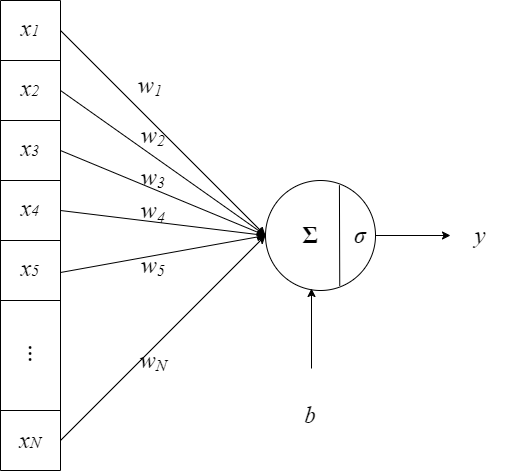
\includegraphics[width=0.5\linewidth]{figures/neuron.drawio.png}
    \caption{神經元示意圖}
    \label{fig:single-neuron}
\end{figure}


結合數個神經元的運算,羅氏(Rosenblatt)於 1958 年 \cite{rosenblatt_perceptron_1958} 提出感知器(Perceptron)模型。根據通用近似定理(Universal Approximation Theorem)\cite{funahashi_approximate_1989} ,感知器理論上可逼近任意函數。然而,後續研究發現單層的感知器具有如「線性不可分」\footnote{例如無法貼合異或(Exclusive OR,XOR)運算等函數} 等先天限制,使其曾經一度不被看好。

為了突破該缺陷,人們嘗試在輸入與輸出層之間增加「隱藏層(Hidden Layer)」,成為「多層感知器(Multilayer Perceptron,MLP)」,如圖 \ref{fig:mlp} 所示。藉助隱藏層的幫助,多層感知器可對輸入進行多次非線性轉換,大大拓展了模型的適用範圍。此模型是透過「加深隱藏層」得來,現今為人們熟知的「深層類神經網路(Deep Neural Network)」即由此得名。

\begin{figure}
    \centering
    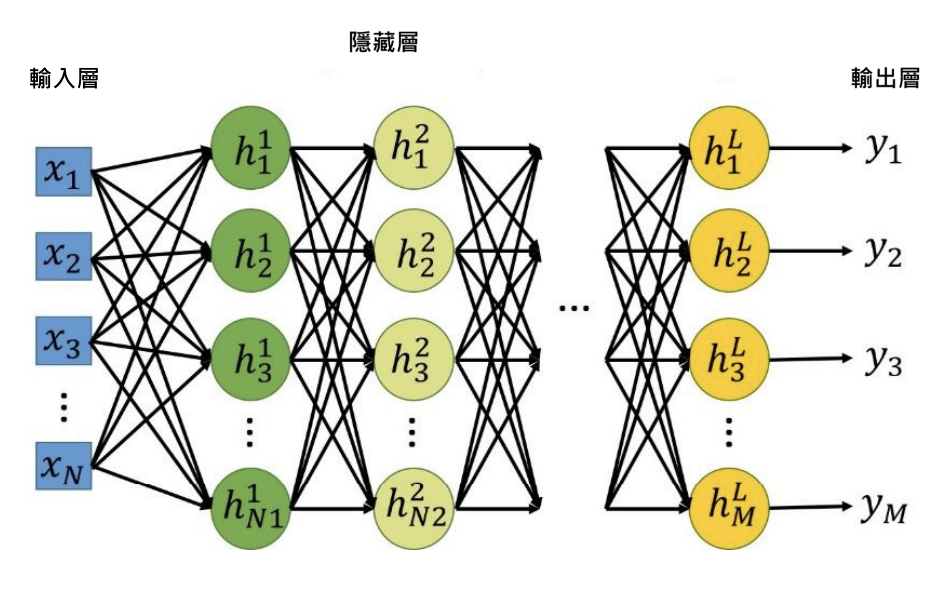
\includegraphics[width=0.8\linewidth]{figures/nnout.png}
    \caption{多層感知器/深層類神經網路示意圖}
    \label{fig:mlp}
\end{figure}


藉助深層類神經網路的彈性,我們可以透過⼤量訓練資料來訓練模型,藉此逼近應⽤任務中欲近似的函數 $f$,該函數蘊藏在資料集 $\mathcal{D} = \{(x_i, y_i)\}_{i=1}^N$ 中,其中每個資料點 $(x_i, y_i)$ 為輸入與輸出間的配對,即對於 $N$ 個資料點都有 $$y_i = f(x_i) \ \  \forall i \in \{1, \cdots\cdots, N\}$$之關係。
為了使這個函數更加逼近目標函數 $f$,
類神經網路會構建一個逼近中的函數 $f_{\theta_t}(\cdot)$ 。
透過不停的迭代,
模型對資料集 $\mathcal{D}$ 的每一筆資料 $x$ 給出預測 $f_{\theta_t}(x)$ 。
透過某個減損函數(Loss Function)$\mathcal{L}$ 計算出誤差(Error),
此誤差對參數 $\theta_t$ 求出梯度(Gradient)後將指示模型更新的方向,
以此乘上學習率(Learning Rate)$\eta$ 後從參數  $\theta_t$ 減去,便能對整個模型進行更新,使之更有機會接近目標函數 $f$。
由於此過程是依照梯度使得函數 $\mathcal{L}$ 逐步降低,以此獲名「梯度下降法(Gradient Descent)」,其公式如下:
$$\theta_{t+1} \leftarrow \theta_{t} - \eta \nabla_\theta\mathcal{L}(\mathcal{D}, f_{\theta_t}(\cdot))$$
其中,$t$ 為當前的迭代數,$\theta_t$ 為當前模型參數,$\theta_{t+1}$ 為更新後的模型參數。

在此模型更新的過程中,減損函數承擔著指引模型逼近的角色,因此根據應用的任務不同,常見的減損函數包括
\begin{itemize}
    \item 均方誤差(Mean Squared Error,MSE):一般用於迴歸(Regression)問題,直接計算兩數值之間的差距的平方和
    $$\mathcal{L}_{\text{MSE}}(y_i, \hat{y}_i) = \frac{1}{N} \sum_{i=1}^{N} (y_i - \hat{y}_i)^2$$

    \item 交叉熵(Cross-entropy,CE):一般用於分類(Classification)問題,著重計算兩個機率分佈之間的差異
    $$\mathcal{L}_{\text{CE}}(y_i, \hat{y}_i) = -  \sum_{i=1}^{N} \left[ y_i \log(\hat{y}_i) + (1 - y_i) \log(1 - \hat{y}_i) \right]$$
\end{itemize}

透過上述的訓練方式可以得知,類神經網路的訓練需要相當龐大且複雜的運算過程,因此剛提出時仍舊難以應用於現實應用中。

為了提高函數貼合的效率,魯氏(Rumelhart)與辛氏(Hinton)等人 \cite{rumelhart_learning_1986, rumelhart_learning_1987} 提出了反向傳播(Backpropagation)演算法,旨在將上述的更新過程,藉助鏈鎖率(Chain Rule)的幫助,由隱藏層逐層反向傳播至輸入層,對整個類神經網路進行修正。

反向傳播演算法的設計,正好能配合圖形處理器(Graphics Processing Unit,GPU)等硬體裝置的優勢,以平行運算能力加速函數貼合(Fit)的效率。由此開始,這種透過深層類神經網路,從大量資料集中發掘函數關係的機器學習演算法,被稱為深層學習(Deep Learning)。 類神經網路在各個領域的泛化能力(Generalizability)已經得到前所未有的效能,包含電腦視覺、語音處理和自然語言處理,因此深層學習在近年成為人工智慧發展的主流。

然而,根據資料特性的不同,並不是所有的資料都適用簡單的「輸入與輸出配對」的模式。研究者根據任務需求,發展出了不同架構的類神經網路以適應資料特性  。
前述最基本的深層類神經網路,由於資料是直接由輸入層,通過逐層的矩陣運算得到輸出,因此被稱之為「前饋式類神經網路(Feed Forward Network,FFN)」。

藉由調整各神經元之間的連接關係,發展出卷積式(Convolutional)、遞迴式(Recurrent)與轉換器(Transformer)類神經網路等架構變體,以適應如影像、語音和文字等不同型態的資料。這些架構在語音與文字處理被普遍使用,接下來將逐一分別介紹:

\subsection{卷積式類神經網路}
  
卷積式類神經網路(Convolutional Neural Network,CNN)為 1998 年由楊氏(Yann LeCun) \cite{lecun_gradient-based_1998} 提出,旨在以訊號處理的卷積(Convolution)運算,模擬生物的視覺皮質感知 \cite{hubel_receptive_1959} 。

\begin{figure}
    \centering
    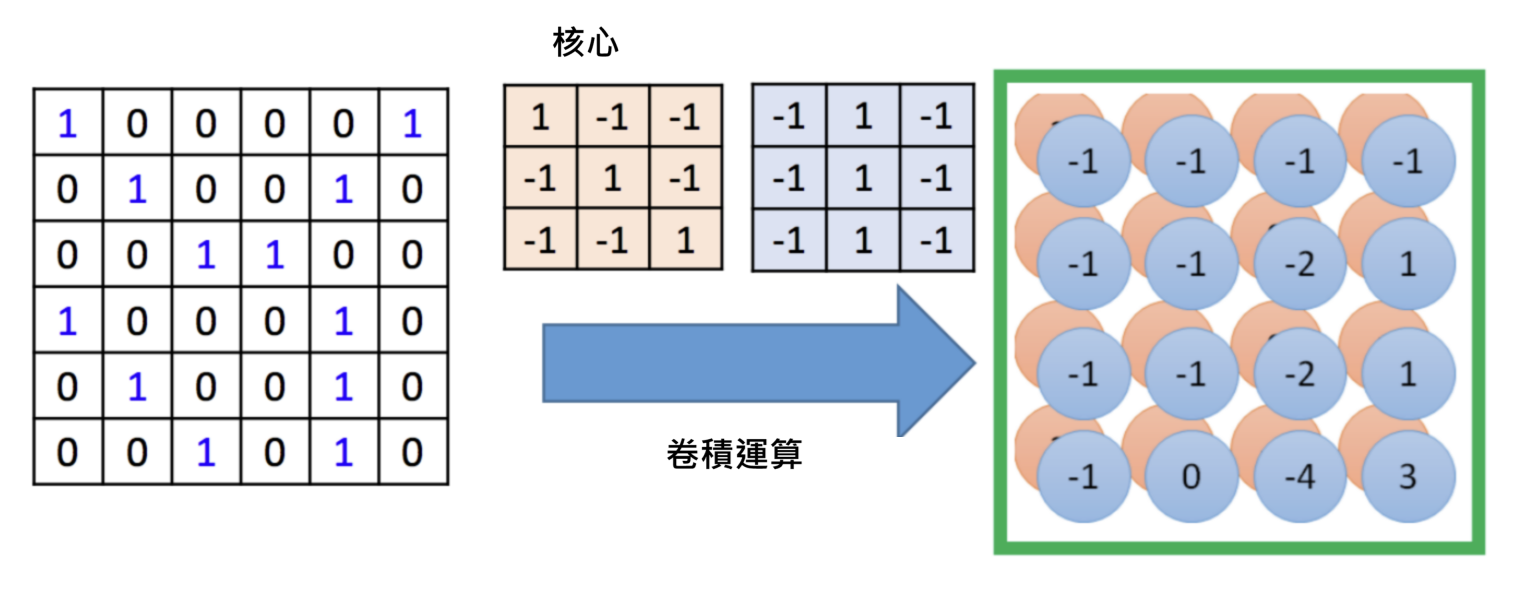
\includegraphics[width=0.9\linewidth]{figures/cnnnew.png}
    \caption{卷積式類神經網路示意圖,取自李宏毅教授的課程投影片}
    \label{fig:cnn}
\end{figure}

如圖 \ref{fig:cnn} 所示,卷積式類神經網路透過核心(Kernel),對輸入的資料 --- 如圖中的二維矩陣 --- 進行卷積運算,獲得該輸入的特徵圖(Feature Map)。核心帶來的移動不變性(Shift-invariance)非常適用於捕捉二維影像中的局部特徵,以作為類神經網路分辨資料的依據。

有別於影像處理中,資料多以二維矩陣表示像素 (Pixel)三原色的亮度數值,因此以二維的卷積運算為主;
由於語音時常處理時間軸之上的訊號,包含聲波波形(Waveform)、時頻譜(Spectrogram)或聲學特徵,因此一維的卷積式模型也時常出現,以模仿人耳聽覺對時變訊號的窗框(Window)的效應,進而觀察到語音中在不同解析度(Resolution)的資訊。


\subsection{遞迴式類神經網路與序列至序列模型}

\subsubsection{遞迴式類神經網路}
  
遞迴式類神經網路(Recurrent Neural Network,RNN)常用於處理隨時間變化的序列資料,特別是語音與文字等等,順序資訊相當關鍵的各種語言任務。

為了處理需要記憶和狀態的資料類型,
遞迴式類神經網路的輸出會重新接回輸入層,
使得前一個時間點(Timestep)的資料與內部狀態
會繼續影響後續的時間點。

常用的遞迴式類神經網路類型有長短期記憶(Long Short-term Memory,LSTM)\cite{hochreiter1997long} 和閘門循環單元(Gated Recurrent Unit,GRU)\cite{cho-etal-2014-properties} 等。

遞迴式類神經網路通常用在處理序列至序列的應用,例如語音辨識、語音合成或機器翻譯等和語言密切相關的任務中。

\subsubsection{序列至序列模型}
  
由於許多語言資料通常以兩個序列互相配對的形式呈現,因此專門處理這類資料的模型被稱為序列至序列模型(Sequence-to-sequence,Seq2seq)\cite{sutskever2014sequence}。此類模型的典型架構由編碼器(Encoder)和解碼器(Decoder)組成,旨在模擬輸入與輸出序列之間的變化與相依關係(Dependency)。

序列到序列模型一般有兩種模式:其一是每個時間點都生成一個輸出的向量,適用於輸入與輸出序列等長的任務,這種模式被稱為符記分類(Token Classification);但更常見的情況是,輸入與輸出序列的長度並不相同。處理後者的典型作法是讓編碼器將輸入序列依據時間,一步一步輸入編碼器,將序列編碼為內部表徵(Latent Representation)。完成編碼後,編碼器將最後一個時間點的表徵代表用以整個序列,稱為「語境向量(Context Vector)」。該向量接著被傳遞給解碼器,依序生成輸出序列。
\subsection{專注機制與轉換器類神經網路}

\subsubsection{專注機制}
  
由於遞迴式類神經網路需要處理整個序列的編碼和解碼資訊,對時間點距離較遠的輸入容易被遺忘,亦即難以處理長期相依性(Long-term Dependency)問題。為了解決這種困境,巴氏(Bahdanau)等人提出了「專注機制(Attention Mechanism)」\cite{bahdanau2014neural}。該機制讓解碼器將每個輸入序列的訊號都視作「部分的」語境向量,由對不同時間點的向量加權合計獲得,使得在生成輸出序列時能依據當時的需求從輸入序列中提取所需的訊息。專注機制的引入,使得序列至序列模型在處理如語音辨識、機器翻譯等任務時大大改善了效能。

\subsubsection{轉換器類神經網路}
  
儘管遞迴式類神經網路善於處理時序資料,但其難以平行化的架構限制了其在訓練和推理(Inference)時的效率。2017 年,瓦氏(Vaswani)等人 \cite{vaswani2017attention} 提出了完全由專注機制構成、不依賴遞迴運算的序列至序列模型,並稱之為「轉換器(Transformer)」,以解決機器翻譯等任務。

轉換器類神經網路一般包含編碼器和解碼器兩部分,均為多層架構。圖 \ref{fig:tfm_arch} 展示完整的轉換器架構圖,以下分別介紹其主要元件:

\paragraph{位置編碼(Positional Encoding)}

對於編碼器或解碼器的輸入序列,模型先對序列中不同位置的時間點進行編碼,取代遞迴式類神經網路逐步運算的過程,使其能在平行計算的同時考慮不同時間點的影響。編碼的函數可依照需求變換,如原始的轉換器採用三角函數進行位置編碼,而在語音模型中,有時也會採用卷積式網路以捕捉輸入的細微資訊。

經過位置編碼後,向量會通過每一個轉換器層(Transformer Layer),進行以多頭專注(Multi-head Attention)為主的一連串運算:

\paragraph{多頭專注}

轉換器層中的專注機制涉及三個輸入向量:詢向量(Query)$Q$、鑰向量(Key)$K$ 和值向量(Value)$V$。專注機制運算如下:
\[
\text{Attention}(Q, K, V) = \text{softmax}
\left(
\frac{QK^\top}{\sqrt{d_k}}
\right)
V
\]
其中 $\text{softmax}$ 為正規化指數函數,$d_k$ 為鑰向量 $K$ 的維度。這一運算首先通過鑰向量和詢向量的內積計算專注權重,而後為避免受維度過大影響而縮小為 $\sqrt{d_k}$ 分之一,最後通過正規化指數函數使得權重總和為 1 ,以此分配給值向量進行加權。

為應對多樣的輸入訊號,每個轉換器層具備多個獨立的專注機制,對三組輸入向量先進行各自不同的 $W^Q$、$W^K$、$W^V$ 線性轉換,稱為「多頭專注(Multi-head Attention)」。對於第 $i$ 個專注頭(Head)有
\[
\text{head}_i = \text{Attention}(QW^Q_i,KW^K_i,VW^V_i)
\]
最後,若有 $h$ 個專注頭,多頭專注模組會將多個頭的結果進行串接(Concatenate),經過線性轉換 $W^O$ 作為模組輸出
\[
\text{MultiHead}(Q, K, V) = \text{Concat}(\text{head}_1, \cdots\cdots, \text{head}_h) W^O
\]

\paragraph{其他層內運算}

每層轉換器層在經過多頭專注運算後,會依序進行以下三個步驟:

\begin{enumerate}
\item 與輸入向量透過殘差連接(Residual Connection)相加,隨後進行層正規化(Layer Normalization)以穩定訓練。
\item 將此結果通過一個簡單的前饋式類神經網路對向量做線性轉換。
\item 再將前饋網路的輸入與輸出再次計算殘差總和後,進行層正規化輸出。
\end{enumerate}

以上為轉換器被提出時的最原始模型,其後對殘差連接、層正規化的安排也存在各類變體。

\paragraph{跨專注機制(Cross-atttention)}

由於解碼器需要來自編碼器的輸入序列資訊幫助輸出,因此,原本在編碼器層中的自專注機制,在解碼器中會再經過一次跨專注機制的運算,使用編碼器提供的詢向量和鑰向量對解碼器的值向量進行專注運算。


\begin{figure}
    \centering
    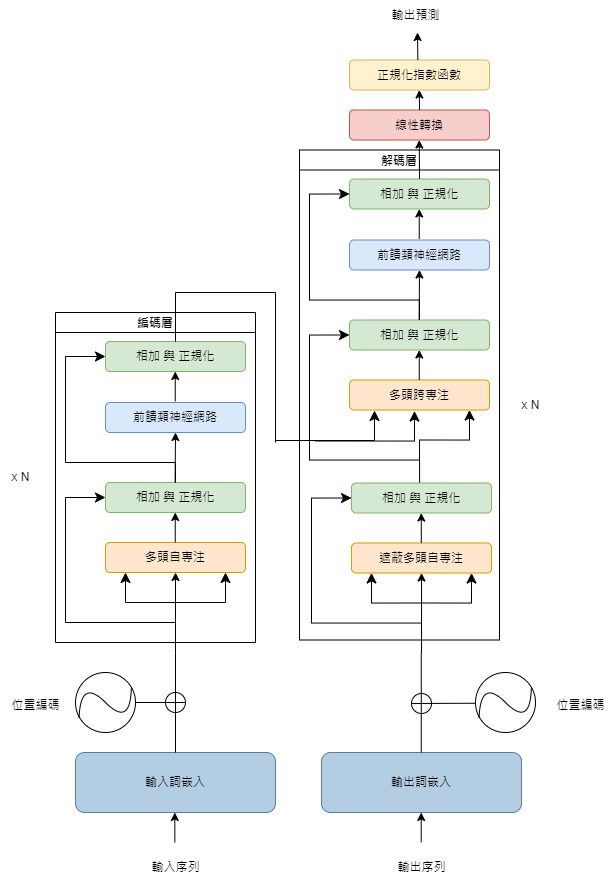
\includegraphics[width=0.9\linewidth]{figures/tfm_arch.drawio.png}
    \caption{轉換器架構圖}
    \label{fig:tfm_arch}
\end{figure}

由於轉換器不需要對每個時間點逐一運算,使其得以實現高度平行化,類神經網路得以透過專注機制同時進行序列資料的大量訓練。這種可擴展性(Scalability)使其在自然語言和語音處理上取得了巨大的進展,近乎取代了原先遞迴式類神經網路的應用場景,近年來甚至被應用在圖像類的資料上\cite{dosovitskiy2021image},展現了此種模型架構的彈性與泛用性,成為目前最前沿的人工智慧主流架構。

除了模型架構,機器學習中不可或缺的另一大部分是對資料的編碼過程。如何更有效率的讓機器理解、處理和輸出資料,是機器學習乃至深層學習的一大課題。面對捉摸不定、抽象且變化萬千的人類語言,語音和文字處理中的表徵學習尤為重要。
\section{表徵與自監督式學習}

\subsection{特徵抽取與表徵學習}
  
不論採用何種模型,為了讓機器可以處理並捕捉輸入資料中的訊號與模式(Pattern),如何對資料編碼和運算的步驟,在機器學習中稱之為特徵抽取(Feature Extraction)或表徵學習(Representation Learning),這是模型建構中不可或缺的重要步驟。

對於抽象的語言概念,早期工程領域根據對語音和文字的理解,分別進行了不同的處理。對於離散且可計數的文字,人們使用詞頻統計衍生出如 n 連詞(n-gram)、TF-IDF(Term-Frequency Inverse Document Frequency)等特徵作為模型學習的前處理步驟;而對於連續且複雜的語音,工程師則透過聲學原理與訊號處理的知識,使用如濾波器組(Filter Bank)、梅爾倒頻譜係數(Mel-Frequency Cepstrum Coefficient,MFCC)等特徵,類比人耳捕捉語音訊號的過程。

在深層學習逐漸發展的過程中,自然語言處理領域的一大里程碑是米氏(Mikolov)提出的「word2vec」模型 \cite{mikolov_efficient_2013},該模型以連續的向量表徵(Vector Representation)取代稀疏(Sparse)的統計數據,對離散的文字單詞進行「詞嵌入(Word Embedding)」編碼。通過大量文本運算,將各單詞之間的共現(Collocation)以跳躍詞(Skip-gram)、連續詞袋(Continuous Bag-of-Word,CBOW)等演算法轉換成高維向量空間中的點,找出每個單詞最適合的語義表徵。爾後,為了更細緻地捕捉同一單詞在不同句子中的脈絡變化,ELMo(Embeddings from Language Model)\cite{peters_deep_2018} 提出了「脈絡化詞嵌入(Contextualized Embedding)」的概念,使得各單詞在運算表徵的過程中可以根據上下文進行些微調整。

\subsection{自監督學習}
  
隨著轉換器模型的提出,BERT(來自轉換器的雙向編碼器表徵,Bidirectional Encoder Representations from Transformers)\cite{devlin_bert_2019} 被提出。通過自專注機制,工程師們無需依賴人工標記,透過預先設定任務(Pretext Task)引導模型從大量文本中自行找出更細緻且考量脈絡(Contextualized)的語義關係,並在許多文字任務上獲得了優異的成績。

自此,楊氏(Yann LeCun)將這種以特定任務作為引導、藉助資料本身的結構替代標註,從大量未標註資料中進行學習資料模式(Pattern)的訓練方式,稱之為「自監督學習(Self-supervised Learning,SSL)」。BERT 的成功使自監督學習得以大行其道,並出現了許多由巨量資料進行預訓練(Pre-train)的基石模型(Foundation Model),有效解決了語言處理領域中的標註資料稀缺的問題。人們在解決語言相關任務時,不需從頭蒐集資料與進行耗時耗能的訓練過程,而是可以利用基石模型優良的泛化(Generalization)能力,解決各種應用任務的需求。相比於預訓練的任務,這些更貼近日常現實的任務被稱為「下游任務(Downstream Task)」,能應對廣泛的下游任務種類,這是基石模型最大的優勢。

有鑑於文字處理方面的成功,語音領域的研究者嘗試將相似模式應用於語音,眾多語音基石模型隨之出現。這些大量的語音資料庫幫助模型萃取出有助於下游任務的語音表徵(Speech Representation),在各種任務上獲得了優於傳統聲學特徵的表現。語音表徵具備的無窮潛力,逐漸成為聲學特徵之外的新選擇。

依照這些語音自監督模型的預訓練學習模式,可大致分為重建式、預測式與對比式模型。以下分別介紹這三類模式:

\subsubsection{重建式學習(Reconstruction Learning)}

此類模型通過對輸入訊號進行擾動(Perturb)後,期望模型將被更動的輸入重新預測回原始資料,通常減損函數表示為:
$$\mathcal{L}_{recon} = \mathbb{E}_x[|f_\theta(\tilde{x}) - x|]$$
其中 $\tilde{x}$ 為擾動後的資料,$f_\theta(\cdot)$ 為模型函數。擾動方式通常以遮蔽為主,在文字處理中以 BERT 為代表,稱為「遮蔽語言模型(Masked Language Model,MLM)」。在語音中,採用此方式學習的有 Mockingjay \cite{liu_mockingjay_2019}、TERA \cite{t_tera_2021} 等模型。  % NPC

\subsubsection{預測式學習(Predictive Learning)}

此類模型通過預訂一些學習目標函數,製造類似輸入與輸出的配對資料,讓模型預測該函數的結果來學習資料中的特定結構。其訓練減損函數可表示為:
$$\mathcal{L}_{pred} = \mathbb{E}_x[\text{eval}(f_\theta(x), \hat{f}(x))]$$
其中 $\hat{f}$ 是期望模型學習的目標函數,$f_\theta(\cdot)$ 為模型函數,$\text{eval}$ 是用來評估預測好壞的標準。

目標函數的典型代表是自迴歸(Autoregressive),期望模型預測未來時間點的輸入表徵。文字方面以生成式預訓練轉換器(Generative Pretrained Transformer,GPT)系列 \cite{radford_language_nodate, brown_language_2020}為代表,語音上的自迴歸預測編碼(Autoregressive Predictive Coding,APC) \cite{chung_generative_2020} 也是採用此種模式。此外,語音基石模型還可以使用其他訓練目標,如 PASE+ \cite{ravanelli_multi-task_2020} 預測其他模型的表徵,而本文著重探究的「隱藏單元 BERT(Hidden-unit BERT,HuBERT)」\cite{hsu_hubert_2021, hsu_hubert_2021-2} 則以預測分群(Cluster)後的輸入表徵為目標,這些預測目標又被視為偽標註(Pseudo-label),後文將著重探討。

\subsubsection{對比式學習(Contrastive Learning)}

此學習方式的訓練目標是要求模型區分正樣本(Positive Sample)與負樣本(Negative Sample)的差異,減損函數通常定義為:
$$\mathcal{L}_{contr} = -\mathbb{E}_x\left[\log
\left(
{\frac
{\sum_{\tilde{x} \in x_{pos}}\exp(\text{sim}(x, \tilde{x}))}
{\sum_{\tilde{x} \in \mathcal{X}}\exp(\text{sim}(x, \tilde{x}))}
}\right)\right]$$

其中 $x$ 為輸入,$x_{pos}$ 為正樣本,$\mathcal{X}$ 為包含正負樣本的資料集,$\text{sim}(\cdot, \cdot)$ 是評估兩個樣本相似程度的函數,常用的相似度函數為內積運算得出的餘弦相似度(Cosine Similarity)。語音上最早使用對比式學習的模型為對比預測編碼(Contrastive Predictive Coding,CPC)\cite{maekaku2022speech},之後如 Wav2vec \cite{schneider2019wav2vec}、Modified CPC \cite{rivière2020unsupervised}、Wav2vec 2.0 \cite{baevski2020wav2vec} 等模型亦是以對比正負樣本的模式訓練,但訓練時正負樣本的定義有所差異,如 Wav2vec 僅以時間維度上相同的向量為正樣本,其餘則將固定時間內的向量皆視為正樣本。

對比式學習通過正負樣本的定義,將預訓練任務形塑為分類問題,因此減損函數本質上為交叉熵,使模型能夠判斷訓練資料中的結構差異。

\subsection{向量量化與離散單元}
  
語音訊號雖然記錄語言資訊,卻與影像資料一樣都是連續數值資料,不像離散的文字較易處理,因此發展出了許多應用廣泛的模型。為了使語音模型訓練可以套用自然語言處理領域的演算法,從連續語音中找出離散表徵逐漸成為研究趨勢,這類研究被稱為「聲學單元發掘(Acoustic Unit Discovery,AUD)」。

由於語言概念本質上是離散符號,向量量化技術常用於涉及語言標註的情境,如電腦視覺經典的量化向量變分自編碼器(Vector-Quantized Variational Autoencoder,VQ-VAE)\cite{van2017neural},利用影像標註的離散語言單詞特性,使模型學習的表徵向量被約束在編碼簿(Codebook) 的幾個向量中。

% 將模型的連續特徵透過甘式軟性最大化和 K-平均兩種向量量化技術
在語音領域,基於 Wav2vec 之上的 Vq-wav2vec \cite{baevski2019vq} 和 Wav2vec 2.0 將連續的語音特徵量化加入訓練目標中,在語音辨識等任務上取得了顯著進步。

HuBERT \cite{hsu_hubert_2021-2} 則應用先對連續的 MFCC 特徵進行 K-平均(K-Means)演算法分群,以所得的群心(Centroid)編號作為訓練目標,實施類似 BERT 的遮蔽語言模型訓練,
並改以此次訓練得到的語音表徵為目標,再次分群後實施第二次訓練。 
這些經過兩輪訓練後,從模型表徵分群得到的群心,被視為「隱藏單元(Hidden Unit)」,編碼了語音訊號中的代表性聲學特徵。透過找出隱藏單元的過程,HuBERT 在低資源情況下達到與 Wav2vec 2.0 相近的語音辨識成績。

\subsection{無文字(Textless)架構}
  
奠基於 HuBERT 等語音基石模型的成功,利用隱藏單元的概念,將大量語音資料表徵進行 K-平均演算法,作為這些語音訊號的偽標籤。如此得到的大量離散隱藏單元形成了「偽文字(Pseudo-text)」的語料庫,基於這些離散單元訓練語言模型,稱為「生成式口語語言模型(Generative Spoken Language Model,GSLM)」\cite{lakhotia_generative_2021-1}。配合反向語音合成訓練基於離散單元的語音生成模型,整體架構不依賴文字標註,訓練出純語音語言模型,稱為「無文字(Textless)架構」\cite{noauthor_textless_2021}。

無文字模式在語音問答(Spoken Question Answering)\cite{lin2022dual}和語音到語音翻譯 (Speech-to-speech Translation)\cite{chen_speech--speech_2023}中取得了前所未有的進展。這些「離散單元(Discrete Unit)」被視為類似文字卻不依賴人類文字標記的語音表徵,具有儲存位元率低和可套用文字語言模型訓練模式的優勢,受到語音社群的廣泛借鑑,後續也帶出了許多如\cite{zhang2024speechtokenizer} 等將語音以離散表徵編碼的研究。

雖然在系統與應用任務上取得了成功,但這些離散單元本身與文字的差異,及其對語音語言模型訓練的幫助,仍是領域內探討的焦點。有鑑於此,本論文基於語言知識,從最接近文字且與語音訊號最相關的「音位(Phoneme)」開始探討,期望了解離散單元能帶來的特徵及其對後續應用的幫助。

\section{本章節總結}
  
本章節首先介紹了深層學習模型的核心部件 --- 類神經網路的基本原理,隨後對本論文研究的核心 --- 「語音表徵」與「離散單元」的發展與歷史進行了梳理。接下來的章節將緊扣這些基石模型得到的離散特徵,對其與「音位」這類語音學標記之間的統計關係進行更深入分析。

%% textless --> 是不是要補一下模型敘述?
% 補 citations
% 順搞,包含表格邊框
% 算 ratio 有必要嗎?
% $$ 長條圖分開討論?
% alignment
% 換 dev

%%% https://arxiv.org/pdf/2102.01192

% mycites
% 最後!處理數據作圖…!! 是要多久……啊就那樣
% phone type

\chapter{單一語音離散表徵與音位的關係}  % 與語音標記的對應模式

  HuBERT \cite{hsu_hubert_2021, hsu_hubert_2021-2} 和 Wav2vec 2.0 \cite{baevski2020wav2vec} 等語音基石模型的成功,
不僅在語音任務上達到了前所未有的表現,
還促進了語音表徵離散化的發展。
由此產生的「無文字(Textless)」架構 \cite{noauthor_textless_2021, lakhotia_generative_2021, lakhotia_generative_2021-1},讓人們在處理語音訊號時,有了連續表徵以外的新選擇。
離散形式的表徵可以直接應用文字領域發展的技術,
如機器翻譯、生成式模型等,為語音技術帶來新的突破。另一方面,基於離散「符記(Token)」的共同形式,
離散語音表徵可以更好的整合文字資料,
促成多模態領域的發展。跨模態離散表徵的成功,
甚至驅使影像領域也開始發展離散表徵,  % 要確認一下「開始」嗎?
如探討唇語的 AV-HuBERT \cite{shi2021learning} 等等,展現了離散表徵在資料處理上的優勢。
  % 不是模型運算
% 還有影像的 vokenization \cite{tan-bansal-2020-vokenization} 等等。好像更早
% TODO: 找到影像那邊的新的 token?

% 語言學那邊只有一般語音?還是包含 acoustic phon 嗎?
此外,除了技術的角度切入,為了探討離散語音表徵成功背後的可能因素,
以及它們與語言學對人類語音理解之間的差異,
甚至是進一步利用這些技術協助更細緻的探討人類的語音現象。
因此,原先在連續語音表徵上的語音學分析,
也開始關注離散表徵在多大程度上能描述語音現象,
將其列入考量,成為除了連續語音特徵和時頻譜之外的另一個選擇。
% TODO: cite  "is cont necessary? 那篇"
% 更由於這些離散表徵形式上和音位、文字的相似性,  %% 這個好像還沒?
%% 他們還是更喜歡 IPA,只是先當成一種新的 label 吧?

\section{相關研究}

\subsection{無文字與離散語音表徵}

  自 HuBERT 帶起的研究之後,
出現了愈來愈多離散表徵相關的研究,
例如 \cite{10097097, abdullah23_interspeech, chang_exploration_2023, liu2024dinosr, zhang2024speechtokenizer, huang2023repcodec} 等等。
它們在提出自己的離散表徵時,
也會採取 HuBERT 的
衡量方式,
% 例如 PNMI 等等的,
來驗證這些離散單元與語音中的內容及人類對語音的詮釋之間
具有一定程度的相關性,
並從資訊理論(Information Theory)的角度,
證明這些離散單元
確實具備區分
不同語音
% 中不同形式的
資訊
的能力
。

\subsection{語音學分析}

  
由於語音處理本身最終是針對人類語音,
因此
有一群研究者通過對人類語音的理解,
將這些知識應用在分析模型如何對語音訊號建構表徵之上。例
如 \cite{deseyssel22_interspeech, wells_phonetic_2022, 10097097, abdullah23_interspeech} 等研究。
% 就韋誠說的妹子那篇嗎?

        基於這些作品
對語音離散表徵的興趣和探討,  % 其實是我的興趣?
本論文也先透過過往幾個常用來分析語音表徵的方式,特別是
HuBERT \cite{hsu_hubert_2021-2} 提出的標準進行初步的分析。
        % 以下介紹此次分析語音表徵的衡量方式:

\section{衡量方式}

  
% 首先是
本次研究主要探討純度(Purity)、熵(Entropy)和相互資訊(Mutual Information,MI)等指標,
這些標準在 HuBERT 中採用 \cite{hsu_hubert_2021, hsu_hubert_2021-2},用於比對機器學習過程中得到的偽標註與人類標註之間的相關性(Correlation)。以下對各標準進行詳細解釋:

        不論是何種語音基石模型,
語音表徵的基本單位是音框(Frame)。因此一段語句(Utterance)的語音離散單元被表示為 $[y_1, \cdots\cdots, y_T]$。其中 $T$ 是該段語句的音框總數。對於該段語句,若給予一段在音框上對齊的語音學標註(Phonetic Label) $[z_1, \cdots\cdots, z_T]$,此時我們可以將離散單元與標註之間配對的出現次數,寫為一個雙變數的共同分佈(Joint Distribution)
    \begin{align}
      p_{yz} = \frac{\sum^T_{t=1}[{y_t = i \wedge z_t = j}]}{T}
    \end{align}

其中 $i$ 是第 $i$ 個音位類別,而 $j$ 指編號為$j$的離散單元。兩個變數的邊際機率(Marginal Probability)分別為
    \begin{align}
    p_z(j) &=\sum_i{p_{yz}(i, j)} \\
    p_y(i) &=\sum_j{p_{yz}(i, j)} 
\end{align}

因此,對於每一個音位 $i$ 而言,這個音位對應最可能的離散單元為
    \begin{align}
      z^\ast(i) = \arg\max_j p_{yz}(i, j)
    \end{align}
與之相對應的,對於每一個離散單元的類別 $j$ 則可以找到機率最高的音位
    \begin{align}
      y^\ast(j) = \arg\max_i p_{yz}(i,j)
    \end{align}

% 於是我們可以計算出以下指標:
透過這些定義,以下分節介紹將要分析的指標:

\subsection{純度}

        本指標考慮音位和離散單元兩個序列之間對應的最高機率,因此從音位與離散單元的角度出發,可以得到以下兩項數據:

\paragraph{音位純度(Phoneme Purity)}

        考慮每個離散單元對應的音位中,最高機率音位的機率,表示為
    \begin{align}
      \mathbb{E}_{p_z(j)}\left[p_{y|z}(y^*(j)|j) \right]
    \end{align}

此指標表示該單元是否對其對應的音位有足夠的代表性。

\paragraph{分群純度(Cluster Purity)}

        與音位純度相對,改以每個音位的角度,考慮對應單元類別的機率
    \begin{align}
      \mathbb{E}_{p_y(i)}\left[p_{z|y}(z^*(i)|i) \right]
    \end{align}

        由於離散表徵進行分群演算法時的類別數是一項超參數(Hyperparameter),且通常離散單元的分群數量會比音位多,因此該統計數據本身不直接具有語音學的解釋意義,而且在分群數量很多時會顯著下降。
然而該指標在考量音位純度時必須一併考慮,
因為當分群數非常多時,分群純度過低
暗示離散單元做不到歸納音位類別的效果,
使得音位純度失去其意義。一個極端的情形是每一個音框都給予不同的離散單元編號,如此音位純度可以達到
         100\%。

\subsection{熵和相互資訊}

  除了純度提供「最高機率」的對應關係,根據 HuBERT 論文 \cite{hsu_hubert_2021-2} 中的分析方式,我們也可以從資訊理論的角度,觀察兩個序列的熵和相互資訊。

\paragraph{熵(Entropy)}

  熵的定義按照資訊理論,衡量兩個序列中標籤類別出現機率的不確定性(Uncertainty),公式寫作:
    \begin{align}
        H(y) &= \sum_i{p_y(i)\log p_y(i)} \\
        H(z) &= \sum_j{p_z(j)\log p_z(j)}
    \end{align}
其中 $H(y)$ 和 $H(z)$ 分別為音位和離散單元的熵,數值愈高分別表示各種音位和離散單元出現的機率愈平均。

\paragraph{以音位標準化之相互資訊(Phone-normalized Mutual Information,PNMI)}

  本數據以「觀察到某一個離散單元,能降低多少音位標註的不確定性」,定義該離散單元的出現背後提供了多少音位的資訊。公式寫為:
    \begin{align}
        \frac{I(y;z)}{H(y)}&=\cfrac{\sum_i \sum_j p_{yz}(i, j) \log \cfrac{p_{yz}(i, j)}{p_y(i)p_z(j)}}{\sum_i p_y(i) \log p_y(i)} \\
        &=\frac{H(y)-H(y|z)}{H(y)} \\
        &=1-\frac{H(y|z)}{H(y)}
    \end{align}

        該項數據愈高,表示離散單元的分群愈能提供語音音位的資訊,是一個品質更好的分群結果。由於離散單元能多好的對應到音位才是人們所關心的問題,因此與純度不同,只以音位的角度出發,而不考慮以離散單元分群的角度。

% \input{3b}

\section{語音學分類(Phone Type)}

% \subsection{簡介}

  除了單一音位本身的特性以外,由於音位之間存在相似的特徵,可以分成幾個組別。
依照 \cite{10097097, abdullah23_interspeech} 的分組方式,對英語的音位進行分類並合併比對數據,
觀察這些離散單元是否有擷取到相似的發聲特徵,而不單純只是把音位分成約 50 類完全獨立的標籤。以下簡介六個音位組別:

% (基於語音表徵本身就是 acoustic sisgnals 來的,應該 by nature 要可以對語音特徵分組吧?)

        % 英語中的音位依照發音的方式,共分成七個類別。

\begin{itemize}
    \item 塞音(Plosive):以完全阻塞氣流的方式發音的音位,包含 /p/、/b/、/t/、/d/、/k/、/g/ 六種
    \item 擦音(Fricative):藉由在口腔中形成的縫隙,使氣流通過時摩擦形成的發音,包含 /f/、/v/、/s/、/z/、/\textesh/ (sh)、/\textyogh/ (如「garage」的 「-ge」)、/θ/ (無聲的 th)、/ð/ (有聲的 th)、/h/ 九種
    \item 塞擦音(Affricate):由塞音和同部位的擦音同時發出的輔音,英語中只有 /t\textesh/ 和 /d\textyogh/ 兩種,即 ch 和 j 的發音
    \item 鼻音(Nasal):使氣流通過鼻腔形成的聲音,有 /m/、/n/、/ŋ/ (ng) 三種
    \item 近音(Approximant):又稱半元音,為介於元音和輔音之間的聲音,有 /j/ (為 y 作為輔音時的發音)、/r/、/l/、/w/
    \item 元音(Vowel):可自成音節的音位,包含發音位置固定的單元音(Monophthong)和會移動的的雙元音(Diphthong),通常以 a、e、i、o、u 字母產生的聲音皆屬於此類別
\end{itemize}


% \paragraph{元音}

% 母音在這邊為了簡單起見,會被分在一起?

% 根據發音的位置是否發生改變,英語的元音可分為:

% \begin{itemize}

% 兩大類別。

% \paragraph{輔音}

% 而輔音按照發音的方式,可分為以下五類:

% \subsection{解釋意義}

% \begin{itemize}
    % \item 純度(Purity):換成以語音學的類別作為新的語音標籤後,有何變化(關聯性更強?)
    % \item 熵(Entropy)(放直方圖解釋) \(\rightarrow\) 語音分類更明顯?
    % \item 對齊(Alignment):是否減少分段資訊的保留(連續子音母音被合併?)
% \end{itemize}

透過將音位分組後,形成新的語音標註,並重新分析統計指標,觀察在純度等數據是否顯示離散單元與語音的發音方式具有更明確的關聯性。


\section{實驗集與分析模型}

%%%%%%%%%
%%%%%%%%%% %%%%%%%%%%%%%%%%
%%%%%%%%%% 本研究的分析對象參考無文字架構 \cite{noauthor_textless_2021, lakhotia_generative_2021, lakhotia_generative_2021-1} 的研究,採用當中提及的 CPC、Wav2vec 2.0 和 HuBERT 三個語音基石模型,並與作為比對的聲學特徵梅爾時頻譜(Mel-Spectrogram),共四種語音表徵模型。模型的詳細資訊如表 \ref{tab:model-info} 所示:
%%%%%%%%%
%%%%%%%%%% \begin{table}
%%%%%%%%%%     \centering
%%%%%%%%%%     \begin{tabular}{|c|l|c|c|} \hline 
%%%%%%%%%%          語音表徵&   模型架構&離散表徵來源層數& 時間解析度(Time Resolution)\\ \hline 
%%%%%%%%%%          HuBERT      &   CNN + Transformer&6& 20 毫秒\\ \hline 
%%%%%%%%%%          Wav2vec 2.0 &   CNN + Transformer&14& 20 毫秒\\ \hline 
%%%%%%%%%%          CPC         &   CNN + GRU&2& 10 毫秒\\ \hline 
%%%%%%%%%%          LogMel      &   聲學特徵&N/A& 10 毫秒\\ \hline
%%%%%%%%%%     \end{tabular}
%%%%%%%%%%     \caption{語音離散表徵的來源層數與音框時間解析度}
%%%%%%%%%%     \label{tab:model-info}
%%%%%%%%%% \end{table}
%%%%%%%%%
%%%%%%%%%% 以下是各語音表徵模型的簡介:
%%%%%%%%%
%%%%%%%%%% \begin{itemize}
%%%%%%%%%%     \item **CPC(對比預測編碼)**:CPC 由編碼器和預測器兩部分組成。編碼器從語音輸入生成嵌入 z。預測器基於過去預測編碼器的未來狀態,系統通過對比損失進行訓練。我們使用 Rivière 和 Dupoux(2020)訓練的 CPC 模型,該模型使用 LibriLight 數據集的6k小時“乾淨”子樣本進行訓練。我們從預測器的中間層提取表示,生成256維的嵌入(每10毫秒一個),如原始論文所述。
%%%%%%%%%%     \item **Wav2vec 2.0**:此模型使用編碼器和預測器,並通過對比性地區分編碼器輸出中的正樣本和負樣本進行訓練。我們使用 Baevski 等人(2020b)訓練的預訓練 Wav2vec 2.0 LARGE 變體,該模型在 LibriLight 數據集的60k小時上進行訓練。此模型將原始音頻編碼為1024維的向量幀(每20毫秒一個)。為了選擇最佳層,我們從模型的每一層提取10小時的 LibriLight 子集的凍結表示,並使用 CTC 損失訓練線性分類器來預測文本標籤的音素版本。第14層在 LS dev-other 上獲得了最低的 PER(Baevski 等人,2021年使用類似的方法選擇了第15層)。
%%%%%%%%%%     \item **HuBERT**:與 CPC 和 Wav2vec 2.0 使用對比損失不同,HuBERT 使用類似於 BERT(Devlin 等人,2019)的掩碼預測任務進行訓練,但輸入是掩碼連續音頻信號。目標是通過對原始語音特徵或早期迭代的學習特徵進行無監督聚類獲得的,這一方法受 DeepCluster(Caron 等人,2018)的啟發。我們使用了 Hsu 等人(2021)訓練的 BASE 12 層變壓器模型,該模型在960小時的 LibriSpeech 上進行了兩次迭代訓練。此模型在每層將原始音頻編碼為768維的向量幀(每20毫秒一個),我們從第6層提取這些向量,如原始論文所述。
%%%%%%%%%%     \item **LogMel**:作為基準,我們考慮使用80個頻帶的對數梅爾濾波銀行編碼器。
%%%%%%%%%% \end{itemize}
%%%%%%%%%% %================


%%%%%%%%%%%%%%%%
  本研究的分析對象參考無文字架構 \cite{noauthor_textless_2021, lakhotia_generative_2021, lakhotia_generative_2021-1} 的研究,
% 採用當中提及的 CPC、Wav2vec 2.0 和 HuBERT 三個語音基石模型,並與作為比對的聲學特徵梅爾時頻譜(Mel-Spectrogram),共四種語音表徵模型。
% 模型的
% 資訊簡述如下:
採用論文中提及的四種語音表徵,簡述如下:

\begin{itemize}
    \item CPC:卷積式編碼器 + 遞迴式預測器,以對比式學習訓練。表徵來自預測器的中間層,每 10 毫秒提取一個向量表徵作為音框
    \item Wav2vec 2.0:卷積式編碼器 + 轉換器預測器,以對比式學習訓練。表徵來自轉換器第 14 層,每 20 毫秒作為一個音框
    \item HuBERT:卷積式編碼器 + 轉換器預測器,以預測式學習訓練,其訓練目標為 K-平均分群演算法的結果,透過遮蔽語言模型的方式訓練。表徵來自轉換器第 6 層,每 20 毫秒作為一個音框
    \item LogMel:為 80 維對數梅爾時頻譜的聲學特徵,在此作為比較基線(Baseline)。音框寬度為 10 毫秒
    
    % CPC 由編碼器和預測器兩部分組成。編碼器從語音輸入生成嵌入 z。預測器基於過去預測編碼器的未來狀態,系統通過對比損失進行訓練。我們使用 Rivière 和 Dupoux(2020)訓練的 CPC 模型,該模型使用 LibriLight 數據集的6k小時“乾淨”子樣本進行訓練。我們從預測器的中間層提取表示,生成256維的嵌入(每10毫秒一個),如原始論文所述。
    % \item Wav2vec 2.0:此模型使用編碼器和預測器,並通過對比性地區分編碼器輸出中的正樣本和負樣本進行訓練。我們使用 Baevski 等人(2020b)訓練的預訓練 Wav2vec 2.0 LARGE 變體,該模型在 LibriLight 數據集的60k小時上進行訓練。此模型將原始音頻編碼為1024維的向量幀(每20毫秒一個)。為了選擇最佳層,我們從模型的每一層提取10小時的 LibriLight 子集的凍結表示,並使用 CTC 損失訓練線性分類器來預測文本標籤的音素版本。第14層在 LS dev-other 上獲得了最低的 PER(Baevski 等人,2021年使用類似的方法選擇了第15層)。
    % \item HuBERT:與 CPC 和 Wav2vec 2.0 使用對比損失不同,HuBERT 使用類似於 BERT(Devlin 等人,2019)的掩碼預測任務進行訓練,但輸入是掩碼連續音頻信號。目標是通過對原始語音特徵或早期迭代的學習特徵進行無監督聚類獲得的,這一方法受 DeepCluster(Caron 等人,2018)的啟發。我們使用了 Hsu 等人(2021)訓練的 BASE 12 層變壓器模型,該模型在960小時的 LibriSpeech 上進行了兩次迭代訓練。此模型在每層將原始音頻編碼為768維的向量幀(每20毫秒一個),我們從第6層提取這些向量,如原始論文所述。
    % \item LogMel:作為基準,我們考慮使用80個頻帶的對數梅爾濾波銀行編碼器。
\end{itemize}


% \ref{tab:model-info} 所示:

% \begin{table}
%     \centering
%     \begin{tabular}{|c|l|c|c|} \hline 
%          語音表徵&   模型架構&離散表徵來源層數& 時間解析度(Time Resolution)\\ \hline 
%          HuBERT      &   CNN + Transformer&6& 20 毫秒\\ \hline 
%          Wav2vec 2.0 &   CNN + Transformer&14& 20 毫秒\\ \hline 
%          CPC         &   CNN + GRU&2& 10 毫秒\\ \hline 
%          LogMel      &   聲學特徵&N/A& 10 毫秒\\ \hline
%     \end{tabular}
%     \caption{語音離散表徵的來源層數與音框時間解析度}
%     \label{tab:model-info}
% \end{table}
我們使用該論文釋出之預訓練模型與 K-平均量化模型。預訓練模型細節詳述於 \cite{lakhotia_generative_2021-1} 中,量化模型則是該篇論文透過公開的 LibriSpeech 資料集 \cite{panayotov_librispeech_2015} 中 train-clean-100 訓練集
,獲取語音表徵後執行 K-平均分群演算法所得,並釋出群數為 50、100 和 200 的三個版本。

% 此後亦跟隨該研究選用特定模型層數及其釋出之 K-平均量化模型。這些模型層數與量化模型在該研究中被證明與語音學特徵最相關,且被使用於無文字架構後續研究之語音離散表徵的抽取方法。無文字研究中 \cite{lakhotia_generative_2021-1} 已透過公開的 LibriSpeech 資料集之 train-clean-100 訓練集
% 語料
% 對四種語音表徵進行 K-平均分群演算法,分別得到群數為 50、100 和 200 的三個量化模型。

        % 本論文以公開的 LibriSpeech 資料集為分析對象,採取其 train-clean-100 為分析的語音語料庫。
        本論文亦以 LibriSpeech train-clean-100 作為分析對象,
% 因此,
% 本研究
將語音語料庫的語音資料經過四個模型獲取連續表徵後,再經過量化模型得到完全由離散單元組成的「偽文字」語料。

        針對語音學的音位標註,透過強迫對齊器(Forced-aligner)\footnote{https://github.com/MontrealCorpusTools/Montreal­Forced­Aligner}的英語預訓練模型,從語料庫的文字轉寫取得語音資料的音位標註與對應的時間範圍。最後透過語音表徵各自的時間解析度生成以音框為單位的音位標註語料。最後將兩者對語音資料集進行音位標註相關性的分析。
%================

\section{分析結果}

%% (((還是放一下長條圖說個事兒好了)))     

\subsection{基於各自音位的分析}

        \begin{table}[!htbp]
            \centering
            \begin{subtable}[t]{\textwidth}
                \centering
                \begin{tabular}{|c|c|c|c|c|c|} \hline 
                                & 音位純度 & 分群純度 & 音位熵 & 離散單元熵 &    PNMI \\ \hline 
                    HuBERT      &   0.5256 &   0.3382 & 3.3152 &     3.8681 & 0.4993 \\ \hline    %% 1.6552 h
                    Wav2vec 2.0 &   0.4006 &   0.2676 & 3.3152 &     3.8215 & 0.3706 \\ \hline    %% 1.2286 w
                    CPC         &   0.5188 &   0.3812 & 3.3146 &     3.7918 & 0.4992 \\ \hline    %% 1.6545 c
                    LogMel      &   0.3253 &   0.1473 & 3.3158 &     3.8630 & 0.2647 \\ \hline    %% 0.8776 l 
                \end{tabular}
                \caption{群數 = 50}
                \label{tab:ch3-clu050}
            \end{subtable}        

            \vspace{0.5cm}        

            \begin{subtable}[t]{\textwidth}
                \centering
                \begin{tabular}{|c|c|c|c|c|c|} \hline 
                                & 音位純度 & 分群純度 & 音位熵 & 離散單元熵 &    PNMI \\ \hline 
                    HuBERT      &   0.6097 &   0.2553 & 3.3152 &     4.5704 & 0.5786 \\ \hline    %% 1.9181 h
                    Wav2vec 2.0 &   0.4877 &   0.2118 & 3.3152 &     4.5284 & 0.4596 \\ \hline    %% 1.5235 w
                    CPC         &   0.5895 &   0.2674 & 3.3146 &     4.5034 & 0.5557 \\ \hline    %% 1.8418 c
                    LogMel      &   0.3348 &   0.0931 & 3.3158 &     4.5591 & 0.2789 \\ \hline    %% 0.9247 l 
                \end{tabular}
                \caption{群數 = 100}
                \label{tab:ch3-clu100}
            \end{subtable}        

            \vspace{0.5cm}        

            \begin{subtable}[t]{\textwidth}
                \centering
                \begin{tabular}{|c|c|c|c|c|c|} \hline 
                                & 音位純度 & 分群純度 & 音位熵 & 離散單元熵 &    PNMI \\ \hline 
                    HuBERT      &   0.6474 &   0.1644 & 3.3152 &     5.2681 & 0.6289 \\ \hline    %% 2.0849 h
                    Wav2vec 2.0 &   0.5427 &   0.1467 & 3.3152 &     5.2173 & 0.5188 \\ \hline    %% 1.7199 w
                    CPC         &   0.6098 &   0.1789 & 3.3146 &     5.1885 & 0.5882 \\ \hline    %% 1.9497 c
                    LogMel      &   0.3474 &   0.0569 & 3.3158 &     5.2322 & 0.2955 \\ \hline    %% 0.9798 l 
                \end{tabular}
                \caption{群數 = 200}
                \label{tab:ch3-clu200}
            \end{subtable}        

            \caption{不同群數在四種基石模型的音位分析數據}
            \label{tab:single-cluster-results}
        \end{table}

  由表 \ref{tab:single-cluster-results} 中可以看出,分群的群數愈多時,音位的純度確實有所上升,但這可能是犧牲分群純度得來的。因此再看 PNMI 的指標可以發現,整體離散單元和音位標註的相關性還是有所提升的。此外,從不同模型來觀察,HuBERT 的表現是四種語音表徵中最好的,一定程度上可以證實 HuBERT 在找出語音中有意義單位上的效能,及其為什麼無文字架構通常以 HuBERT 作為抽取語音離散表徵的模型。

\subsection{基於語音學分類的分析}

        \begin{table}[!htbp]
            \centering
            \begin{subtable}[t]{\textwidth}
                \centering
                \begin{tabular}{|c|c|c|c|c|c|} \hline 
                                & 標註純度 & 分群純度 & 標註熵 & 離散單元熵 &     NMI \\ \hline 
                    HuBERT      &           0.7466 &   0.1422 &         1.7530 &     3.8681 &  0.5742 \\ \hline    %% h  1.0065
                    Wav2vec 2.0 &           0.6913 &   0.1570 &         1.7530 &     3.8215 &  0.4682 \\ \hline    %% w  0.8208
                    CPC         &           0.7418 &   0.1953 &         1.7530 &     3.7918 &  0.5644 \\ \hline    %% c  0.9894
                    LogMel      &           0.5980 &   0.0953 &         1.7530 &     3.8630 &  0.3403 \\ \hline    %% l  0.5966 
                \end{tabular}
                \caption{群數 = 50}
                \label{tab:ch3-clu050}
            \end{subtable}        

            \vspace{0.2cm}        

            \begin{subtable}[t]{\textwidth}
                \centering
                \begin{tabular}{|c|c|c|c|c|c|} \hline 
                                & 標註純度 & 分群純度 & 標註熵 & 離散單元熵 &     NMI \\ \hline 
                    HuBERT      &           0.7804 &   0.0856 &         1.7530 &     4.5704 &  0.6148 \\ \hline    %% h  1.0778
                    Wav2vec 2.0 &           0.7219 &   0.0889 &         1.7530 &     4.5284 &  0.5252 \\ \hline    %% w  0.9207
                    CPC         &           0.7790 &   0.0997 &         1.7530 &     4.5034 &  0.6046 \\ \hline    %% c  1.0599
                    LogMel      &           0.6032 &   0.0567 &         1.7530 &     4.5591 &  0.3512 \\ \hline    %% l  0.6157 
                \end{tabular}
                \caption{群數 = 100}
                \label{tab:ch3-clu100}
            \end{subtable}        

            \vspace{0.2cm}        

            \begin{subtable}[t]{\textwidth}
                \centering
                \begin{tabular}{|c|c|c|c|c|c|} \hline 
                                & 標註純度 & 分群純度 & 標註熵 & 離散單元熵 &     NMI \\ \hline 
                    HuBERT      &           0.8004 &   0.0464 &         1.7530 &     5.2681 &  0.6563 \\ \hline    %% h  1.1504
                    Wav2vec 2.0 &           0.7490 &   0.0527 &         1.7530 &     5.2173 &  0.5671 \\ \hline    %% w  0.9941
                    CPC         &           0.7947 &   0.0644 &         1.7530 &     5.1885 &  0.6345 \\ \hline    %% c  1.1123
                    LogMel      &           0.6107 &   0.0335 &         1.7530 &     5.2322 &  0.3652 \\ \hline    %% l  0.6401 
                \end{tabular}
                \caption{群數 = 200}
                \label{tab:ch3-clu200}
            \end{subtable}        

            \caption{不同群數在四種基石模型按照語音學類別的分析數據}
            \label{tab:single-cluster-phonetype-results}
        \end{table}
        將表 \ref{tab:single-cluster-phonetype-results} 與音位的表 \ref{tab:single-cluster-results} 進行比較,能看出音位數據表現的趨勢,也能在語音類別中看出來。然而,由於語音類別數明顯少於音位的種類數,因此語音類別標註的純度相較音位會較高。


\section{本章總結}

  本章節探討以音框為單位取出的語音離散表徵與對應的音位標註之間的關係,從分析結果中可以看到,HuBERT 模型的離散表徵確實與人類理解的語音單位「音位」之間具有最明顯的相似性,也進一步證明
% 以此尋找語音中的
為何 HuBERT 是抽取語音離散表徵時最常使用的模型。

%%% 其實數據有點 bug,/h/ 跟元音不分單雙

然而,單一離散表徵僅能代表 10 或 20 毫秒的語音訊號,而音位的長度經常佔據不只一個離散表徵。因此,下一章節將進一步組合多個離散表徵成為符記,分析它們與音位之間的關係。

\chapter{多個語音離散表徵與音位的關係}
\newcommand{\myhline}{\noindent\makebox[\linewidth]{\rule{\paperwidth}{0.4pt}}}

\newcommand{\draftbegin}{\centerline{\textcolor{magenta}{\textbf{=======================以下是草稿!=======================}}}}
\newcommand{\drafttermi}{\centerline{\textcolor{blue}{\textbf{=======================以上是草稿!=======================}}}}



\section{動機}
  
% 如前一章所述,由於單一離散單元所代表的僅為 10 或 20 毫秒的語音訊號,而作為一種類似文字的語音內容表示,每一個音位往往都對應超過一個以上的離散單元。因此,基於使得離散單元序列可以不論在長度和對應的語音訊號兩方面都能更接近於文字,因此從自然語言處理的分詞演算法(Tokenization)得到靈感,本章節將嘗試將這些演算法應用於離散單元的序列之上,並應用上一章節的分析方式,比對將多個離散單元重新分組形成符記之後,是否可以在保有「完全從語音訊號獲得」的同時,得到更接近於音位的序列。
如前一章所述,一個文字或音位往往對應到上百毫秒的語音訊號,然而單一離散單元所對應的聲音訊號為 10 或 20 毫秒,亦即同一段語音所對應的離散單元數目將比音位或文字多出許多。本章節從自然語言處理中獲取靈感,將分詞演算法(Tokenization)應用於離散單元序列上,並應用上一章節的分析方法檢驗將多個離散單元所組成之符記。探討分詞後,離散單元是否可以同時擁有無文字(Textless)\cite{lakhotia_generative_2021, lakhotia_generative_2021-1, noauthor_textless_2021} 的特性,且更接近音位的序列,成為更好的語音表徵。
%   
% (1) 20B-21A (2) 21B-22A (3) 22B-23A (4) 23B-24A

\section{相關研究} 
  
在無文字架構被提出後的約兩年後,藉分詞方法組合離散單元的研究逐步出現。
最初提出「聲學片段(Acoustic Piece)」的是任氏(Ren)等人 \cite{ren_speech_2022}\citetag{1-22A4-Pretrain-ap}),該論文
% 基於離散單元與音位的關聯性,並透過
% 觀察
% 從
比對
離散單元序列
及對應的文字轉寫,
% 之間的,
% 中,對應轉寫文字的單詞,兩者互相比對可以
從中
觀察
到許多相似的模式(Pattern),
而且不限於單一語者
。
% ,甚至在不同語者之間也能觀察到此一現象。
% 以此
受此啟發,
本論文
首先將離散單元使用句子片段(SentencePiece) \cite{kudo_sentencepiece_2018} 分詞,獲得新的符記 --- 「聲學片段(Acoustic Piece)」,並用於語音辨識的預訓練上。

不久,由吳氏(Wu)提出的 Wav2seq \cite{wu_wav2seq_2023}\citetag{2-22A5-wav2seq}論文中,考量文字與語音的序列長度差異,並基於離散單元和音位的關聯性,將離散單元視為字符(Character),嘗試將這些字符透過分詞方法組成「偽語言(Pseudo-language\footnote{偽語言對應之離散單元被視為「偽文字(Pseudo-text)」})」,來幫助語音到文字的模型。因為解碼器在實際應用時需要生成的序列多是文字的符記 --- 次詞單位(Subword Unit),因此該篇研究旨在讓模型在預訓練
% 時可以更適應下游任務。
後可以快速適應下游任務。
與前一篇呼應,「聲學片段」對語音預訓練的效果在
\cite{10096788}\citetag{3-23A-coarser-grain}
中被探討,
此後聲學片段更被應用於
縮短資料序列長度\cite{chang_exploration_2023}\citetag{4-23B-Exploration of Efficient End-to-End ASR using Discretized Input from Self-Supervised Learning} 
、
語音生成
\cite{shen2024acoustic}\citetag{5-24A-speech-gen},
或
% 透過離散單元與可以分離語者資訊的能力學習表徵
學習更穩健(Robust)的語音表徵
\cite{chang2023r}\citetag{6-23B-rspin-acousticpiece}。

% \cite{yang2024towards}\citetag{23B-toward-universal-speech-distok-asrtts}
% \cite{ma23b_interspeech}\citetag{23A-pusinglimit}

近期,張氏(Chang)等人\cite{chang_exploring_2024}\citetag{7-23B-shinji-hsiuhsuan}將以分詞方法處理離散單元的流程(Pipeline)納入 ESPNet 套件 \cite{watanabe2018espnet} 中,並在語音辨識、語音翻譯等任務中獲得了超越以往的表現,進一步證明了這個方法的效果。

% \textbf{\#\# 對語音離散表徵的分詞研究}
% \subsection{(Version ChatGPT)}
% \section{分詞方法在語音處理中的應用}
% 在語音處理領域,這些分詞方法同樣適用。通過對離散語音單元的分詞處理,可以有效地將語音信號轉換為子詞單元,提高語音識別和翻譯模型的性能。例如,Ren 等人的方法通過句子片段化處理將高頻代碼模式合併為聲學片段,從而有效地將輸入音頻與自然語言橋接起來 \cite{ren_speech_2022}。


\section{分詞方法}

  
在以文字為主體的自然語言處理中,文字文本除了以單詞(Word)或字元(Character)為處理單位,更常見的作法是
透過
分詞演算法(Tokenization)將
文本
分段,以「次詞單位(Subword Unit)」構成詞彙表
來重新編碼文本,用於文字模型的訓練與推理。

分詞方法的優點一般包含:

\begin{enumerate}
    \item 固定詞彙表大小,避免未登錄詞(Out-of-vocabulary,OOV)
    \item 縮短資料序列的長度,提升訓練和推論的效率。
    \item 分解單詞,捕捉更細緻的語意關係,模擬如英語中的字首(Prefix)、字尾(Suffix)等等具有特定意義的文字組合。
\end{enumerate}

\subsection{常見演算法}

  
以下介紹幾種常見的分詞方法:

\paragraph{位元組對編碼(Byte Pair Encoding,BPE)}

位元組對編碼 \cite{10.5555/177910.177914, sennrich_neural_2016} 是一種常用的分詞方法,最初來自資料壓縮技術 \cite{10.5555/177910.177914},後來被引入到自然語言處理領域,用以處理機器翻譯問題 \cite{sennrich_neural_2016} 。
該演算法從字元開始,根據詞彙表中各個次詞單位的頻率,反覆合併常見的字元成為新的次詞單位,直到達到預定的詞彙表大小。

% BPE 的基本思想是通過反覆合併頻繁出現的字節對來構建子詞單元。其主要優點包括:


% \begin{enumerate}
%     \item 減少詞彙表的大小:BPE 通過將常見的子詞單元加入詞彙表,顯著減少了詞彙表的大小,提高了模型的泛化能力。
%     \item 處理罕見詞和新詞:通過使用子詞單元,BPE 能夠更好地處理罕見詞和新詞,因為這些詞可以拆分為已存在的子詞單元。
%     \item 減少數據冗餘:BPE 在減少數據冗餘方面表現出色,提升了訓練和推理的效率。
% \end{enumerate}


% \draftbegin
% \input{4-3-tokenization}
% \drafttermi
\paragraph{單詞片段(WordPiece)}

WordPiece \cite{wu2016google} 演算法由 Google 用以訓練機器翻譯系統,並在 BERT \cite{devlin_bert_2019} 模型中被使用而廣為人知。與 BPE 同樣是透過反覆合併的策略,但合併的依據改以機率模型取代出現頻率。

\paragraph{單一詞語言模型(Unigram Language Model)}

單一詞語言模型 \cite{kudo2018subword} 是基於語言模型的分詞方法,以機率分佈選擇次詞單位,並以最大化輸入文本的機率來為文本分段。


\subsection{句子片段(SentencePiece)套件}

  
SentencePiece \cite{kudo_sentencepiece_2018}
是由 Google 開發的分詞套件,實作了前述的 BPE 和單一詞演算法。其優勢在於可應用於不同語言,尤其用於處理中文、日文等不使用空格分隔單詞的語言文本時,此套件大大的簡化了前處理的流程。


\input{scripts/before/4after}

% \mychcnt{5}
\chapter{結論與展望}
\section{研究貢獻與討論}
\section{未來展望}

% \newpage
% \



% \newpage
\ % The empty page
\newpage
% \newpage
% \
% \newpage

% % this file is encoded in utf-8
% v3.0 (Jun. 11, 2019)

%%% 參考文獻
\newpage
\phantomsection % for hyperref to register this
\addcontentsline{toc}{chapter}{\nameRef}
\renewcommand{\bibname}{\protect\makebox[5cm][s]{\nameRef}}
%  \makebox{} is fragile; need protect
\bibliographystyle{IEEEtran}  % 使用 IEEE Trans 期刊格式
\bibliography{thesis}


%%% 附錄
%\input{my_appendix.tex}

%%% 自傳
%\newpage
%\chapter*{\protect\makebox[5cm][s]{\nameVita}} % \makebox{} is fragile; need protect
%\phantomsection % for hyperref to register this
%\addcontentsline{toc}{chapter}{\nameVita}
%\input{my_vita.tex}



% <<<
\newpage
\phantomsection % for hyperref to register this
\addcontentsline{toc}{chapter}{\nameRef}
\renewcommand{\bibname}{\protect\makebox[3.5cm][s]{\nameRef}}  % fixed by JEFF
% \renewcommand{\bibname}{\protect\makebox[5cm][s]{\nameRef}}  % original
%  \makebox{} is fragile; need protect
\bibliographystyle{IEEEtran}  % 使用 IEEE Trans 期刊格式
\bibliography{citations,scripts/zz}

% >>>

\end{document}
